\documentclass[11pt,letterpaper]{article}
\usepackage{cogsys}
\usepackage[T1]{fontenc}
\usepackage{times}
\usepackage{graphicx}
\usepackage{booktabs}
\usepackage{amsmath}
\usepackage{natbib}
\setlength{\bibsep}{0.20ex}

% Postulate environments, as in the ACS 2026 paper.
\newcounter{rpostulate}
\newcounter{opostulate}
\newcounter{ppostulate}
\newcounter{lpostulate}
\newenvironment{rpost}{\stepcounter{rpostulate}\par\noindent\hangindent=21pt\hangafter=1
  \textbf{R\therpostulate.}~\ignorespaces\setlength{\parindent}{0pt}\setlength{\parskip}{4pt}}{\par\smallskip}
\newenvironment{opost}{\stepcounter{opostulate}\par\noindent\hangindent=21pt\hangafter=1
  \textbf{O\theopostulate.}~\ignorespaces\setlength{\parindent}{0pt}\setlength{\parskip}{4pt}}{\par\smallskip}
\newenvironment{ppost}{\stepcounter{ppostulate}\par\noindent\hangindent=21pt\hangafter=1
  \textbf{P\theppostulate.}~\ignorespaces\setlength{\parindent}{0pt}\setlength{\parskip}{4pt}}{\par\smallskip}
\newenvironment{lpost}{\stepcounter{lpostulate}\par\noindent\hangindent=21pt\hangafter=1
  \textbf{L\thelpostulate.}~\ignorespaces\setlength{\parindent}{0pt}\setlength{\parskip}{4pt}}{\par\smallskip}

\newcommand{\trellis}{\textsc{Trellis}}

\cogsysheading{X}{2026}{1-26}{12/2026}{X/2027}
\ShortHeadings{Concepts and Chunks from Raw Experience}{K.\ Singaravadivelan and P.\ Langley}

\begin{document}

\title{Learning Concepts and Chunks from Raw Experience}

\author{Karthik Singaravadivelan}{ksingara3@gatech.edu}
\author{Pat Langley}{patrick.w.langley@gmail.com}
\address{Georgia Institute of Technology, Atlanta, GA 30332 USA; \
         Institute for the Study of Learning and Expertise,
         2164 Staunton Court, Palo Alto, CA 94306 USA}

\begin{abstract}
Chunking replaces many parts with one symbol, and expertise comes from a better code.
We present the second version of \trellis{}, a cognitive system that learns two linked
Cobweb hierarchies, one of concepts and one of chunks, from a stream of experiences with
no parse trees, labels, or gradients. The system parses by summing over every
segmentation its memory allows, generates from the same memory, and learns by storing each
candidate chunk with its posterior probability as a weight. We apply it to children's stories and
to chess, and we present most of the evidence as case studies of real output.
From 250 to 1,000 training sentences \trellis{} writes new grammatical sentences about as often as a matched LSTM.
It writes them more often than a matched GPT at 250 and 500 sentences, a result that does not hold at 1,000
sentences on four confirmation seeds. Both neural models lead at 4,000 sentences.
In chess, relational chunks code positions on unseen squares in fewer bits than byte-pair coding over squares
and in about as many as byte-pair coding over shapes. Recall of chess positions rises with experience
in the order Chase and Simon found for people, but it rises on random positions as well, where people do not improve.
A search for a setting that yields grammatical but meaningless output found none.
%% PENDING r225: language compression (bits per token against n-grams, BPE and neural models) will go here once measured; until then the abstract makes a compression claim for chess only.
\end{abstract}

\section{Introduction}

People hold about seven items in working memory at once \citep{miller-magical-seven}, or about four
when rehearsal and grouping are controlled \citep{cowan-magical-four}. Yet chess masters
reconstruct far more of a middle-game position than beginners do after five seconds of study
\citep{chase-simon}. The masters do not hold more items. They hold
larger ones: each recurring configuration of pieces is a single chunk, so
twenty-six pieces fit in a handful of slots. On random boards the advantage shrinks to a small residual that
persists, which indicates that the units come from experience with the domain
\citep{gobet-simon-random}. We read these findings as a statement about
compression. A chunk is one symbol for many parts, and expertise is a better code.

A second kind of structure complements chunks. A concept is one description
for many instances that behave alike. A single concept can cover \textit{dog},
\textit{cat}, and \textit{bird} wherever they fill the slot in ``the \_\_\_ ran.'' Chunks save symbols
by naming parts that occur together, whereas concepts save description by grouping
instances that behave alike. Neither saves much alone. A system with chunks and no concepts
cannot relate a new chunk to older ones, and a system with concepts and no chunks
has only single tokens to group \citep{langley-concepts-chunks}.

\citet{singaravadivelan-langley-acs} proposed a theory that links the two. \trellis{}
keeps a taxonomy of concepts organized by the contexts in which elements occur and
a taxonomy of chunks organized by their parts. It ties the two
by naming each chunk's parts with concepts from the first taxonomy. That paper tested the theory on
small synthetic grammars. The system learned from sentences paired with
sample parse trees and parsed greedily, one candidate pair at a time. It left three questions open: whether a less greedy parser could repair the choices a greedy one gets wrong,
whether chunks could be learned from the raw token stream alone, and whether the theory extends to natural text and to chess.

Version 2 of \trellis{} addresses all three, and the answers differ in strength.
The system reads a raw stream of experiences and uses gold labels only to score its output.
It parses by inside-outside computation over every binary segmentation of an experience.
It generates one element at a time using a score for everything the rest of the experience could still become.
It learns by storing every candidate chunk, weighted by the probability the parse assigns to it.
The two linked taxonomies stay as they were. The answer on parsing is negative. On sentences of at most eight words, a greedy parse
produces the same trees as the full computation in 93\% of cases, with the same agreement with a shallow-phrase reference and the same
discrimination of broken sentences, at a fifth of the cost. We use the full computation because it is cheap at this length and
supplies the posterior weights that learning stores. Whether those weights matter more than the best tree, and whether the full computation pays on longer inputs, remains untested.
The answers on raw streams and on new domains are positive but bounded, and the rest of the paper reports them.
We foreground case studies of real parses, generated sentences, chunk histories, chess chunks,
and a recall trial after Chase and Simon, and we add learning curves and four core metric tables.

\textbf{Contributions.} We present an unsupervised, incremental, gradient-free
learner of concepts and chunks that parses and generates from one memory. We show that, with 250 to 1,000 training sentences, its generations
match those of an LSTM and exceed those of a GPT at two of three sizes.
We locate where it falls behind as data grow and offer an untested hypothesis about why.
We characterize the chunks it finds in children's stories, including how
consistently independent learners find them and how often its trees differ from right-branching.
In language its chunk inventories agree across seeds less than raw frequency does. We show that
its chess chunks encode recognizable chess ideas, code shifted positions as compactly as a shape-based byte-pair coder,
and reproduce the ordering of Chase and Simon's recall results with one divergence that we document.
We report a negative result: a dial that varies how abstract the generator's words are
yields meaningful output at one end and word salad at the other, but no setting that yields
syntactic output without meaning.
%% PENDING r225: if language compression is measured and supports it, add a sentence to the contributions and restore a compression statement in the title.

\section{Concepts and Chunks in \trellis{}}

Version 2 keeps the representation and organization postulates of version 1, which we restate because every result depends on them.
Cobweb \citep{fisher-cobweb}
builds a taxonomy of probabilistic concepts incrementally and without labels. Each instance
is a set of attribute-value pairs, and each concept stores a distribution over the values of
every attribute. The system sorts a new instance down the tree by a criterion
called category utility.

\trellis{} applies Cobweb to experiences made of elements in relations, following
the representation of \citet{maclellan-cobweb-language} for language. In a sentence, the elements are words and the
relation is adjacency. An element is either a primitive, such as a word, or a composite, which we call a chunk.
Every element has a \textit{context} description, the window of
tokens on either side of its span, and every composite has a \textit{content}
description, which names its two parts.

\begin{rpost}
Elements are primitives or composites. A composite's content description names its two parts,
and every element has a context description that records its surroundings.
\end{rpost}

\begin{rpost}
A composite's two parts are named by concepts in the context taxonomy,
so the content taxonomy never sees a surface word.
\end{rpost}

\begin{opost}
Long-term memory contains a content taxonomy that organizes composites by their parts.
\end{opost}

\begin{opost}
Long-term memory contains a context taxonomy that organizes every element, primitive or composite, by the surroundings in which it occurs.
\end{opost}

The two taxonomies give each element two descriptions that do not interfere, and the second representation postulate
links them. Because a chunk names its parts by concept, one chunk description covers
every instance whose parts belong to those concepts. Figure~\ref{fig:hierarchies} shows leaf-level subtrees of
both taxonomies from version 1 and the links between them, and Figure~\ref{fig:instances}
shows one primitive and one composite instance.

\begin{figure}[!t]
\centering
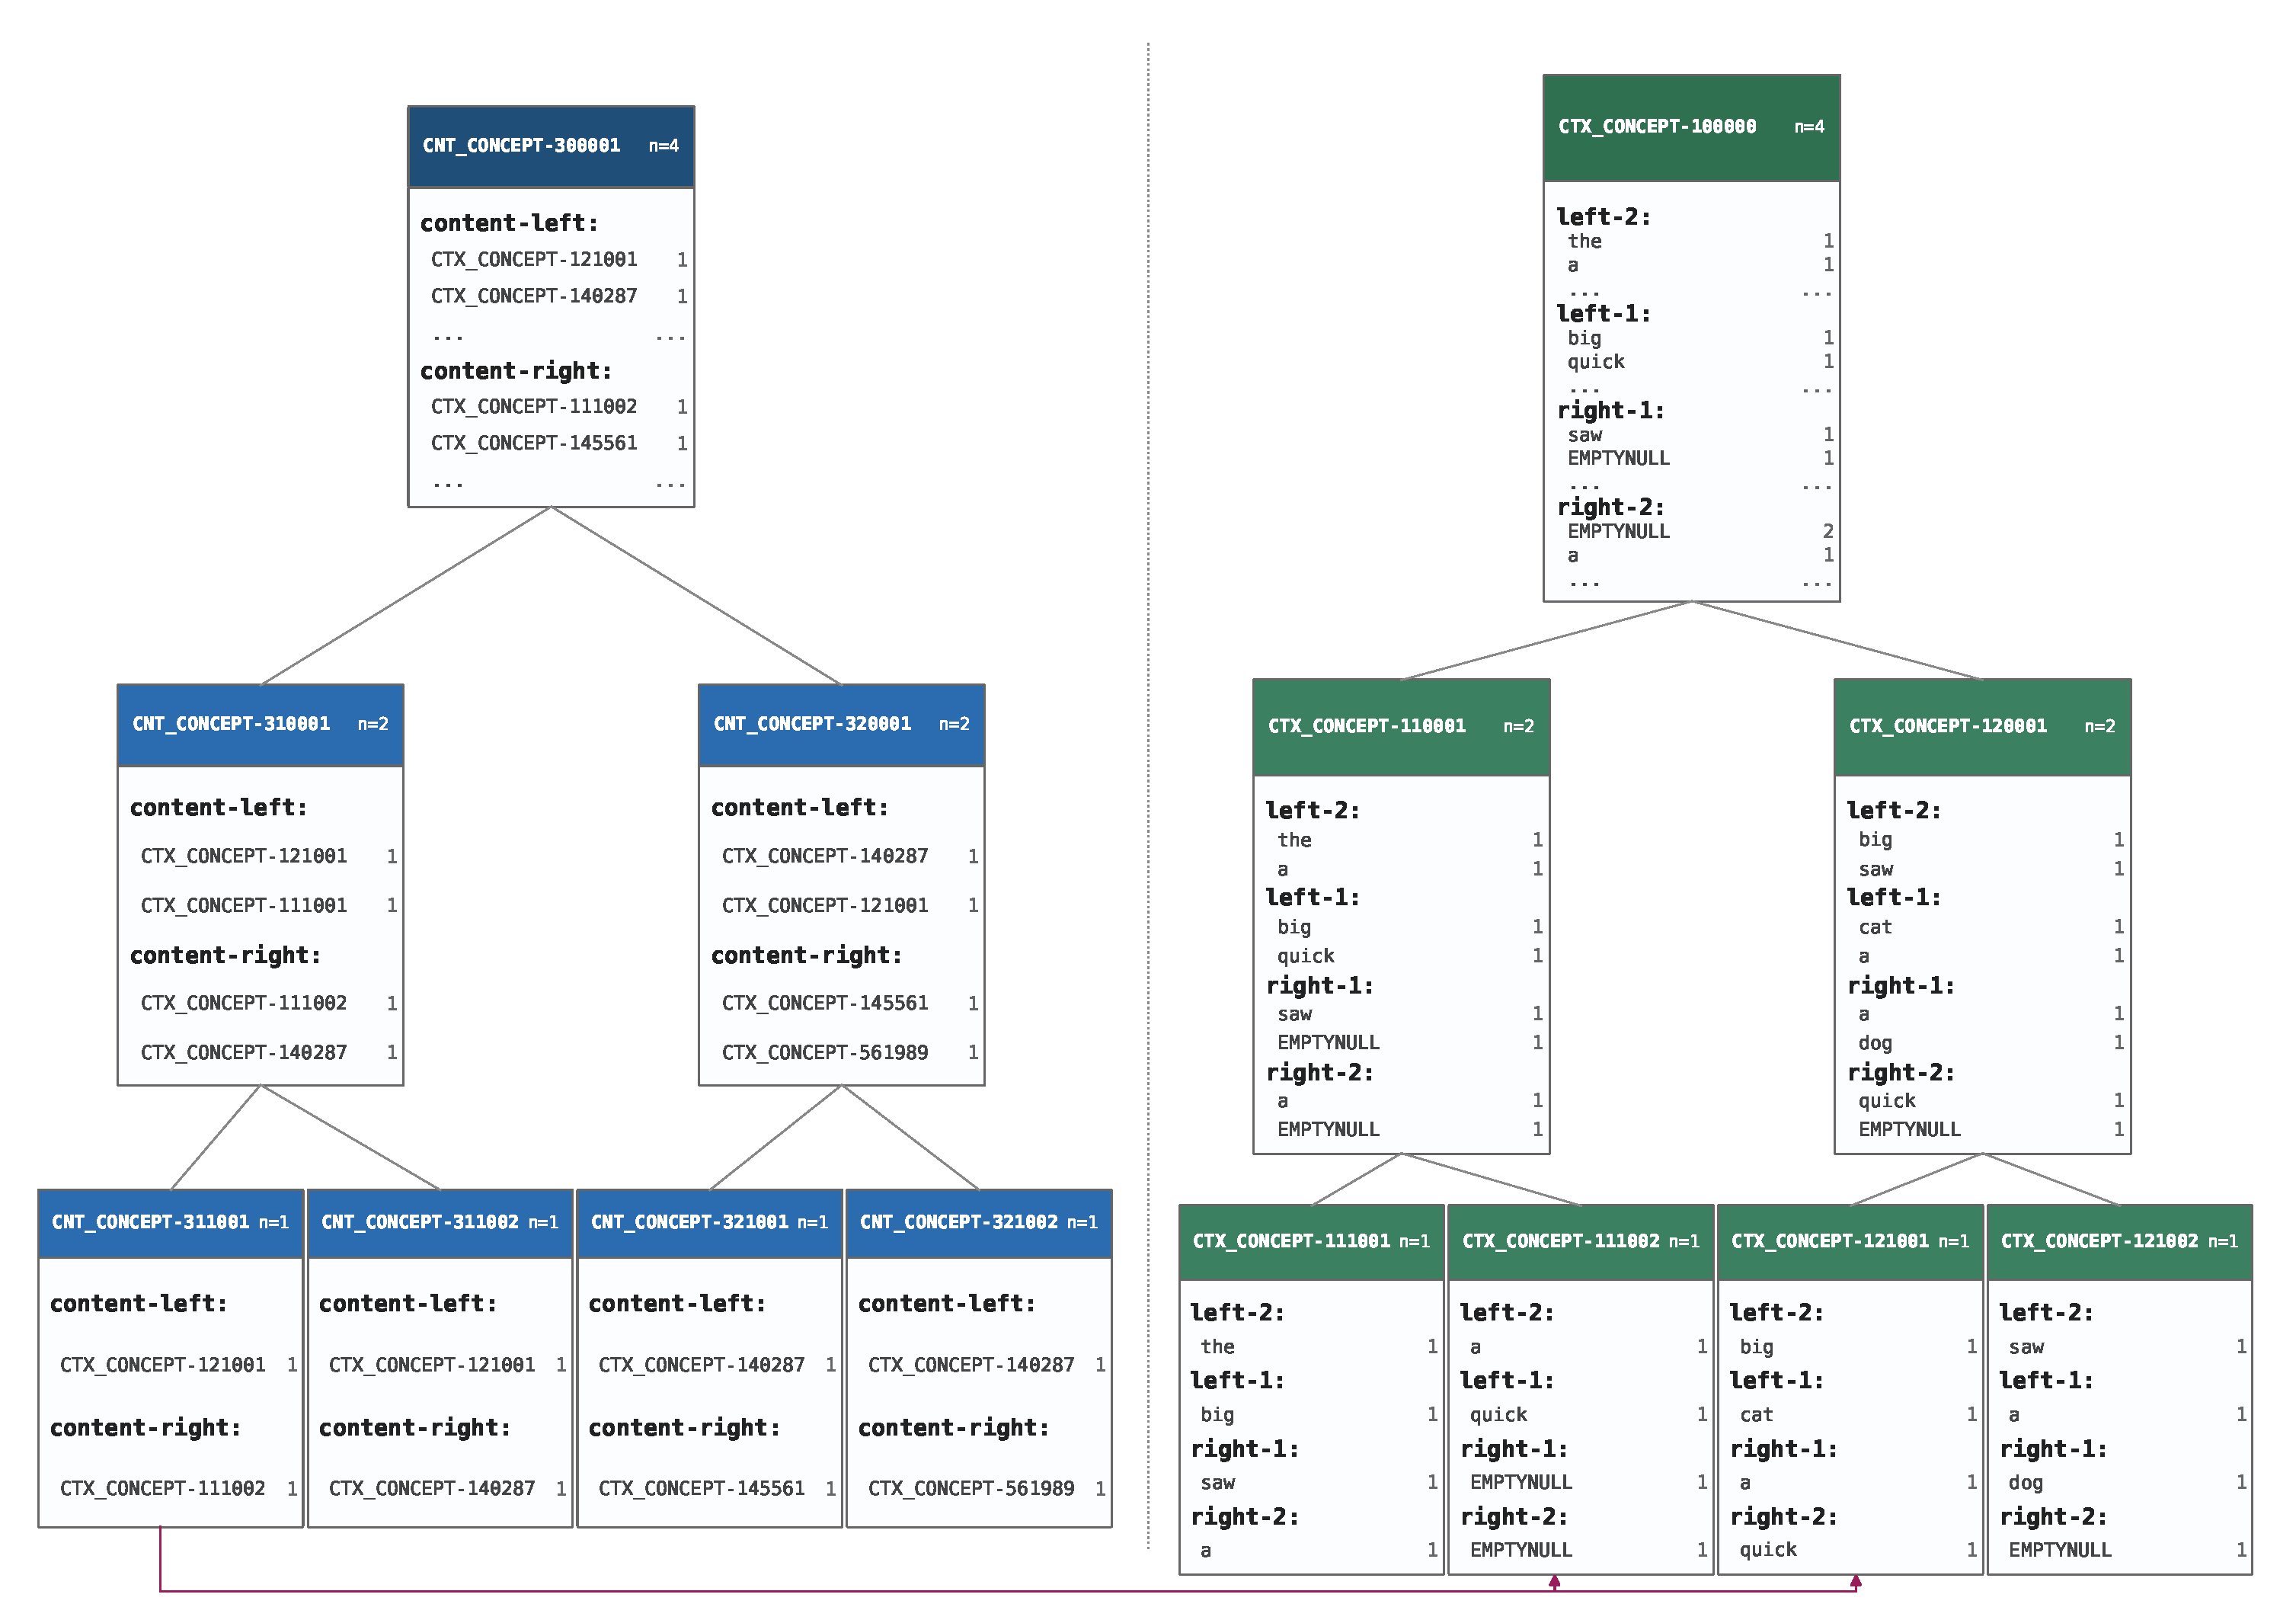
\includegraphics[width=0.9\textwidth, trim=0 0 15 15, clip]{figures/hierarchies}
\caption{Leaf-level subtrees of the content taxonomy (left) and the context taxonomy
(right) from the first version of \trellis{} (synthetic grammar, trained from sample parses).
Arrows mark the cross-taxonomy link: a content leaf names its children by context concepts.
Version 2 uses the same structure.}
\label{fig:hierarchies}
\end{figure}

\begin{figure}[!t]
\centering
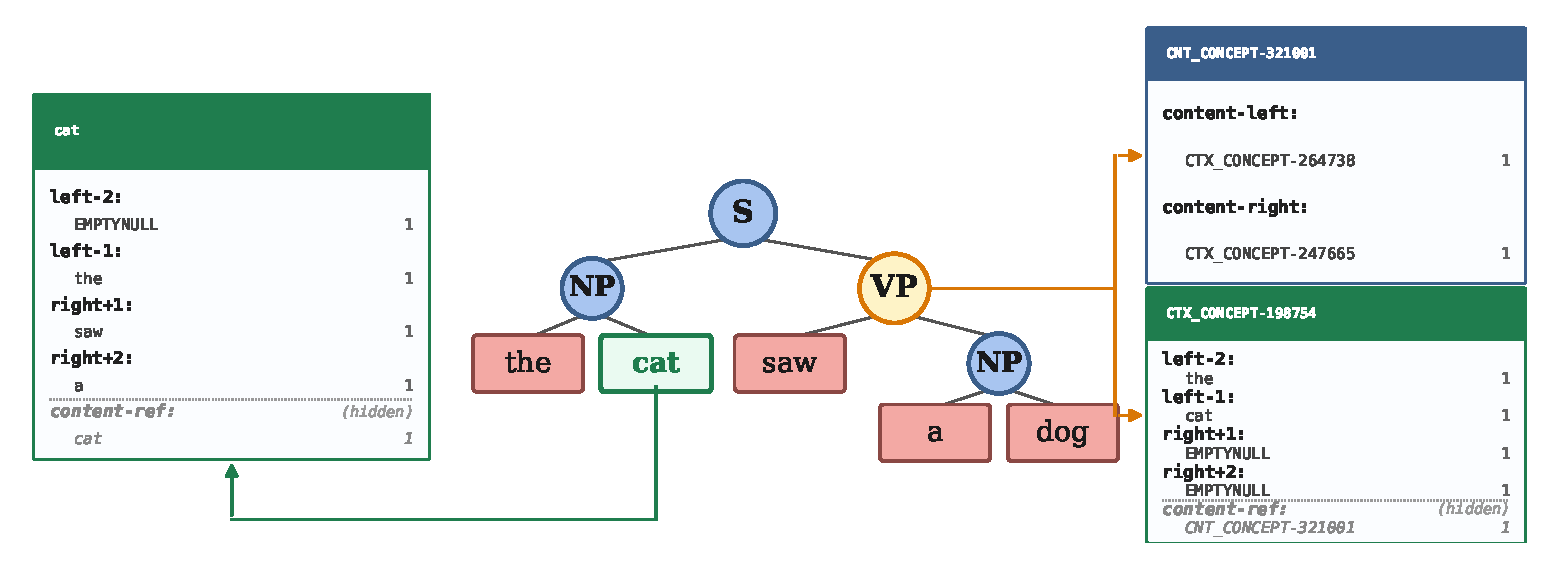
\includegraphics[width=0.9\textwidth]{figures/instances}
\caption{One primitive (``cat'') and one composite (``saw a dog'') from a parse of
``the cat saw a dog.'' Each box header gives the concept to which the instance was sorted.
The composite's content description points into the context taxonomy.}
\label{fig:instances}
\end{figure}

\section{Parsing, Generation, and Learning in Version 2}

Version 2 changes the performance and learning mechanisms, which we state as three further postulates.

\begin{ppost}
Parsing sums over every binary segmentation of an experience. An inside pass
scores each span from its sub-spans, and an outside pass scores everything around it.
The system reports the segmentation with the most expected correct chunks.
\end{ppost}

Version 1 proposed candidate chunks over adjacent pairs, admitted those that cleared a
recognition threshold, and committed the best one, so a wrong early choice could not
be undone. Version 2 scores every candidate span. The inside-outside algorithm
\citep{lari-young} converts these scores into a posterior for every span, and the reported tree maximizes the
expected number of correct spans, the criterion of \citet{goodman-metrics}.
The sentences we parse are short, so full inside-outside is cheap.

\begin{ppost}
Generation writes one element at a time. Each element is chosen with
a score that sums over every chunk that could surround its position, so the element sees chunk
context in both directions.
\end{ppost}

The generator proceeds in four steps. It reads the stored statistics of the taxonomies, takes the prompt as context, chooses a length, and fills each position by
drawing from the stored word-in-context counts at the context concept, weighted by the outside score of
the position. A pair gate restricts draws to word pairs that memory has seen side by side, and an exact-boundary
rule lets a sentence begin or end only with words that began or ended a stored sentence. A window
width and a sampling temperature set how far the output departs from stored sentences.

\begin{lpost}
Every candidate chunk enters both taxonomies, weighted by its posterior probability. The memory that parses
sentence $n$ is the memory built from sentences 1 to $n-1$.
\end{lpost}

Learning remains incremental and unsupervised, as in Cobweb. No separate routine creates chunks:
parsing proposes candidates, and learning treats them as data. Because the parse of each sentence uses only
earlier sentences, the system never reads a gold tree and never makes an offline pass. Table~\ref{tab:v1v2} summarizes the
differences between the two versions.

\begin{table}[t]
\caption{Differences between the first version of \trellis{} \citep{singaravadivelan-langley-acs}
and version 2. The representation and organization postulates are unchanged.}
\label{tab:v1v2}
\begin{center}
\small
\begin{tabular}{lll}
\toprule
 & Version 1 & Version 2 \\
\midrule
Input & sentences with sample parse trees & raw token stream \\
Parsing & greedy, bottom up, recognition threshold & inside-outside over every span \\
Generation & top-down expansion with recall thresholds & one word at a time, outside-weighted \\
Learning & committed chunks only & every candidate, weighted by posterior \\
Domains & synthetic grammars & children's stories, chess \\
\bottomrule
\end{tabular}
\end{center}
\end{table}

\section{Implementation}

The implementation realizes each postulate with a small number of quantities. A candidate span $s$ receives a weight
\begin{equation}
w(s) = 2^{\,g(s)/\tau}, \qquad g(s) = \log_2 \frac{(n_{c^*}/n_0)\,P(s \mid c^*)}{P(s \mid c_0)},
\label{eq:weight}
\end{equation}
where $c^*$ is the concept under which the span sorts, $n_{c^*}/n_0$ is that concept's share of all experiences, $c_0$ is the root,
and the gain $g$ combines the values computed in the two taxonomies. The temperature $\tau$ controls how sharply the weights favor high-gain spans.
The posterior of a span is the weight of the analyses that contain it divided by the weight of all analyses,
\begin{equation}
\mu(s) = \frac{\sum_{t \ni s} \prod_{s' \in t} w(s')}{\sum_{t} \prod_{s' \in t} w(s')},
\label{eq:posterior}
\end{equation}
computed by the inside and outside passes, and the reported tree maximizes $\sum_{s \in t} \mu(s)$.
Learning stores each candidate in both taxonomies with count $\mu(s)$.

During generation, a candidate word is drawn with probability proportional to its stored count at the context concept times
$\exp\bigl((z-z_{\max})/T\bigr)$. Here $z$ is the log of the outside score of the position given that word, and $z_{\max}$ is the largest such log score among the candidates.
At a high sampling temperature $T$ the draw follows the stored counts alone, and at a low temperature the outside score dominates.
Generation temperature $T$ and learning temperature $\tau$ are separate settings. Table~\ref{tab:config} lists every configuration of the system that this paper uses
and the results that depend on each.

\section{Experimental Design}

\paragraph{Domains and preprocessing.} Our language data come from TinyStories \citep{eldan-tinystories}. Stories arrive split into sentences and words, and we keep sentences of
three to eight words drawn from a 250-word vocabulary. The held-out stories never enter training. Each
model learns $n$ training sentences for $n$ from 125 to 4,000. The input is a token stream that is
pre-segmented and restricted to a small vocabulary, and \textit{raw} here means that the system sees no tags, trees, or labels.
For chess we use positions from Lichess games, taken at ply 30 in the idea and move studies, and we test on positions from held-out games.
A position arrives as a set of pieces on squares, and the system derives offsets and relations between pieces from that set.

\paragraph{Evaluation sets.} Two held-out sets of real sentences appear below. Set S is a shared 400-sentence set that serves the chunk and parse-tree studies,
which use the memory of the generation recipe (configuration C3 in Table~\ref{tab:config}). Set C comprises, for each seed, 300 real sentences from that seed's own held-out stories, together with
400 further held-out sentences that calibrate thresholds, and it serves the broken-sentence studies (configuration C4).
Numbers computed on the two sets differ for the same quantity, such as right-branching agreement (.49 on set S, .42 on set C), and every table and caption names its set.

\paragraph{Baselines.} We compare \trellis{} with n-gram models, an LSTM \citep{hochreiter-lstm}, and a small GPT-style
transformer \citep{vaswani-attention}. All models train on exactly the same $n$ sentences. For each seed and size we choose a neural model's size by
held-out loss on sentences from stories the stream never reached. The grid covers 1, 2, or 4 layers, widths 64, 128, or 256, and dropout .1 or .3 for the GPT,
and 1 or 2 layers, widths 128 or 256, and the same dropout for the LSTM. Training uses AdamW with early stopping (patience six, at most 80 epochs).
We did not record parameter counts. We sample each neural model at a tuned temperature. At low temperature a neural model repeats its training data (2 to 14\% of draws are distinct at temperatures .1 to .3), which would hand \trellis{} an unfair advantage.
An n-gram sampler emits only stored n-grams, so it scores zero on the fair count below by construction. We report n-gram models only in the parsing studies.
For chess compression we compare with byte-pair encoding \citep{sennrich-bpe} over squares and over shapes, with Krimp \citep{vreeken-krimp}, and with the general-purpose compressor xz.

\paragraph{Questions and measures.} The studies address five questions in order.
Q1 (commission) asks whether \trellis{} writes new, grammatical sentences as often as neural models trained on the same data.
Q2 (omission) asks whether its scores accept real held-out sentences and reject broken ones.
Q3 asks which chunks it finds and how consistent they are across independent learners.
Q4 asks whether its chess chunks carry chess structure, compress positions, and reproduce the pattern of Chase and Simon's recall results.
Q5 asks whether one setting of the generator can move its output among meaningful, syntax-only, and nonsense regimes.
Following the grammar-induction methodology of \citet{grids-langley-stromsten}, Q1 measures errors of commission, because a generated sentence that is ungrammatical or stored is a failure,
and Q2 measures errors of omission, because a real sentence that a score rejects is a failure.

\paragraph{Generation protocol.} Each model writes sentences, and a language-model judge decides whether each is
grammatical, and the training stream tells us whether it is new. The \textit{fair count} is the number of
distinct, new, judged-grammatical sentences that contain a trigram the training stream never stored, divided by the number
of attempted draws. Repeated and copied sentences count against the generator, because a model that repeats a few grammatical sentences would otherwise look good.
We use eight seeds. Seeds 13, 17, 19, and 23 selected the settings, and seeds 29, 31, 37, and 41 confirm them. We report both groups.
A seed fixes which stories supply the training sentences. Training sets overlap across seeds by 8 to 14\% of sentences, so seeds are not independent samples.
We report paired differences with 95\% $t$ intervals and, for the confirmation group, bootstrap intervals.
We call two models level when the interval for their difference includes zero and has a lower bound above $-.03$. We fixed this margin in advance, and it equals roughly a tenth of the fair count.
The default judge is Qwen2.5-3B \citep{qwen25}, which passes .89 of real held-out sentences.
The \trellis{} sampling temperature enters the generation rule above. Its grid extended beyond the neural grids after its optimum at 250 sentences sat on the edge.

\paragraph{Parsing protocol.} Gold parses are scarce for children's stories, so we ask whether a
score accepts real held-out sentences and rejects sentences we have broken in controlled ways. The broken
classes are scrambles, a single swap of adjacent words, and a swap of every content word with another of the same part of
speech and verb frame, which leaves the sentence grammatical but unsensible. We fix each score's threshold so that it accepts 90\% of 400 real calibration sentences,
and we report the share of each broken class that it still accepts, so lower is better. We use four seeds. We compare
trees with a shallow-phrase reference from NLTK and with the right-branching tree.

\paragraph{Judging syntax and meaning.} The regime study needs a judge that separates syntax from meaning.
Two language models, Qwen3-8B \citep{qwen3} and phi-4 \citep{phi4}, each answer a syntax question and a meaning question, and we
average their logits. We set thresholds on one half of the control sentences and report the other half.
This ensemble judges the regime study only. The generation comparison uses the single-axis Qwen2.5-3B judge, so its conclusions depend on that judge;
a second judging of the same draws is in progress.

\section{Evaluation in Language}

We begin with real output and turn to metrics afterwards.

\subsection{Parses of real sentences}

Table~\ref{tab:cases} shows parses of held-out sentences by four learners that each trained on its own 1,000 sentences (configuration C3, set S).
Protocol: we show the trees of all four seeds for a sentence, next to the NLTK reference, and we state whether the sentence was chosen or drawn.

\begin{table}[t]
\caption{Parses of held-out TinyStories sentences (set S, 400 sentences) by four \trellis{} learners (seeds 13, 17, 19, 23), each trained on its own 1,000 sentences, next to the NLTK shallow-phrase reference.
The first two groups were chosen by reading the candidates for linguistic plausibility, and the third group was drawn at random from the 262 seed-13 trees that are neither right- nor left-branching (draw seed 213, indices 110, 314, 163, 219).
The last sentence was chosen because all four learners parse it the same wrong way.}
\label{tab:cases}
\begin{center}
\footnotesize
\begin{tabular}{p{0.20\textwidth}p{0.10\textwidth}p{0.58\textwidth}}
\toprule
Sentence & Learner & Tree \\
\midrule
\multicolumn{3}{l}{\textit{Chosen}} \\
the tree had no friends & seed 13 & [[the tree] [[had no] friends]] \\
 & seed 17 & [[[the tree] had] [no friends]] \\
 & seed 19 & [[the tree] [had [no friends]]] \\
 & seed 23 & [[[[the tree] had] no] friends] \\
 & reference & [the tree] [had [no friends]] \\
one day tom went to the park & all four seeds & [[[[one day] tom] went] [to [the park]]] \\
 & reference & [one day] [[tom went] [to [the park]]] \\
\midrule
\multicolumn{3}{l}{\textit{Drawn at random (seed 13)}} \\
one day he saw a big ball & seed 13 & [[[[one day] he] saw] [a [big ball]]] \\
 & reference & [one day] he [saw [a big ball]] \\
the girl was happy to help & seed 13 & [[the girl] [was [happy [to help]]]] \\
 & reference & [the girl] [was happy] [to help] \\
she ran fast to get the cake & seed 13 & [[[she ran] fast] [to [get [the cake]]]] \\
 & reference & she [ran fast] [[to get] [the cake]] \\
i will help you said tom & seed 13 & [[i will] [help [you [said tom]]]] \\
 & reference & i [[will help] you] [said tom] \\
\midrule
\multicolumn{3}{l}{\textit{Systematic error}} \\
suddenly the little girl had an idea & all four seeds & [[[[suddenly the] little] girl] [had [an idea]]] \\
 & reference & suddenly [the little girl] [had [an idea]] \\
\bottomrule
\end{tabular}
\end{center}
\end{table}

Only the chunk ``the tree'' appears in all four trees of the first sentence. Seed 13 groups ``had no,'' seed 17 attaches the subject to the verb first, seed 19 matches the reference, and seed 23 builds a left-leaning tree.
The second sentence receives one tree from all four learners. It treats ``one day'' and ``the park'' as chunks, as the reference does,
and attaches the subject to the verb before the prepositional phrase. Two of the four drawn trees look good. In the fourth, the sentence has two clauses, ``i will help you'' and ``said tom,'' and the learner joins ``you said tom'' across the clause boundary.
The last row shows that consistency across learners can coincide with error. The pairs ``suddenly the'' and ``the little'' are both frequent, so every seed builds the noun phrase from left to right and never forms ``the little girl.''
Independent learners agree on the bracket set of held-out sentences at F1 of .65, .70, and .72 after 250, 500, and 1,000 sentences (set S), where random binary trees give .34 on an earlier 300-sentence set.
A learner with the recipe of the parsing-curve study (configuration C4) gives a cross-seed F1 of .87 at 1,000 sentences on seed 13's 300 set-C sentences, so the two agreement figures come from different learners and different sets.

\subsection{Trees that are not right-branching}

English trees lean right, so a parser can score well by always branching right. After 1,000 sentences, 82\% of the held-out parses of \trellis{} differ from right-branching, and 66\% are neither right- nor left-branching (set S).
Where they differ they score .28 to .32 F1 against the NLTK reference, below right-branching on the same sentences (.45 to .48). We make no claim that the departures are better.
The reference contains only shallow phrases and favors
right-branching trees, so it cannot credit structure that the linguist's convention does not mark. On the full set S \trellis{} scores .32 to .39 F1 across seeds against .49 for right-branching.
On set C the corresponding values for the C4 learner are .35 for \trellis{} and .42 for right-branching, and 96\% of its trees differ from right-branching.

\subsection{Chunk biographies}

Chunks persist while their concepts change. Table~\ref{tab:bio} follows four chunks of seed 13 (configuration C3) through training.
Protocol: for each chunk we count the training sentences, up to each checkpoint, whose learned tree bracketed that word string, and we list the company the chunk keeps in the content taxonomy at 250 and 1,000 sentences.
The chunk ``the bird'' first appears at sentence 27 in seed 13 and in seed 19, at sentence 37 in seed 23, and at sentence 59 in seed 17. Its first example in seed 13 is ``the bird saw a big cat.''
After 250 sentences it shares a concept with ``all day,'' ``had fun,'' and ``very happy.'' After 500 it shares one with ``he was,'' ``he liked,'' and ``they played,'' and after 1,000 with ``happy too,'' ``the animals,'' and ``the tree.''
A concept in an incremental taxonomy contains whatever the learner has seen so far, and ``the bird'' keeps different company at every checkpoint.
In seed 17 the chunk ``tim was'' shares a concept at 250 sentences with ``sue was,'' ``tom was,'' and ``sara was,'' a clean concept of a name followed by a form of \textit{be}.
The fixed opener ``one day'' keeps company with other openers and subject chunks, and with neither ``every day'' nor ``all day.''

\begin{table}[t]
\caption{Four chunks of one \trellis{} learner (seed 13, TinyStories, configuration C3): the sentence at which each was first bracketed by a learned tree, the number of training sentences whose tree bracketed it by 100, 250, 500, 750, and 1,000 sentences,
and other chunks in the same content concept at 1,000 sentences.}
\label{tab:bio}
\begin{center}
\footnotesize
\begin{tabular}{llcp{0.43\textwidth}}
\toprule
Chunk & First & Counts & Same concept at 1,000 sentences \\
\midrule
the bird & 27 & 2, 5, 8, 13, 14 & happy too; the animals; was inside; with tim; the tree; feel better \\
one day & 250 & 0, 0, 4, 8, 9 & at the; he knew; inside the; as he; the little; he played \\
tim was & 32 & 2, 4, 7, 12, 19 & one day; they said; they found; she put; he walked; the park \\
in the park & 194 & 0, 1, 4, 7, 11 & in the sun; with his friends; his friends outside; her friend tom; with the bear; with his ball \\
\bottomrule
\end{tabular}
\end{center}
\end{table}

Figure~\ref{fig:chunkcases} follows six held-out sentences through five training sizes, and Figure~\ref{fig:chunkcurves} compares the share of committed chunks that are noun, verb, and prepositional phrases with chance.
Two-word strings dominate the chunks the learners find. They include a determiner and a noun, a subject and an auxiliary, a name and ``and,'' and fixed time words such as ``one day'' and ``every day.''
Fourteen chunks appear in the top 50 of all four seeds, including ``one day,'' ``he wanted,'' ``the bird,'' ``the cat,'' and ``the dog.''
Chunk inventories overlap across seeds far more than chance would predict (a Jaccard overlap of .33 for the 50 most frequent chunks, against .01 to .03 by chance).
The overlap is lower than that of raw n-gram frequency (.51) or byte-pair encoding (.43) on the same data. In language, chunking adds no cross-seed agreement beyond frequency, and we found no language result in which chunking outperforms a frequency baseline.

\begin{figure}[!t]
\centering
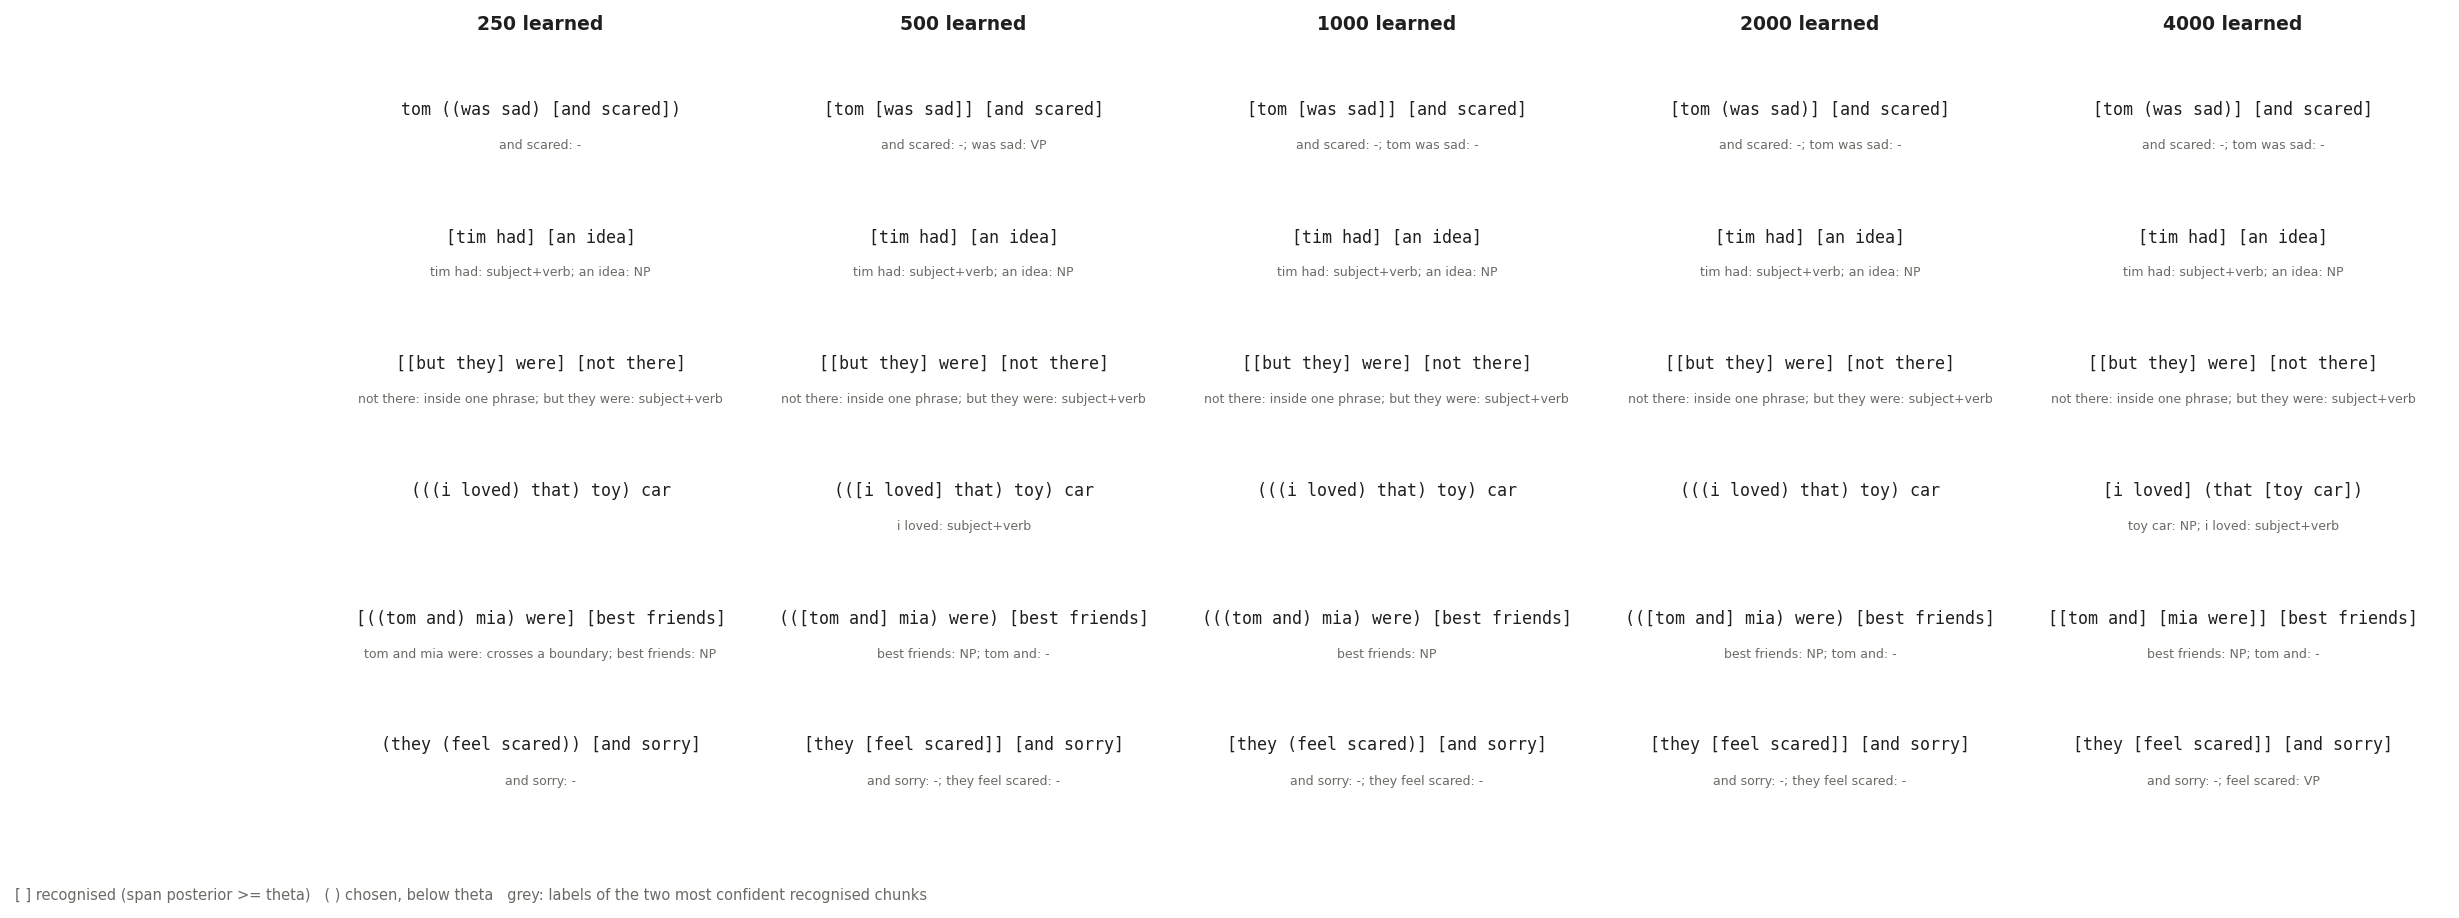
\includegraphics[width=\textwidth]{figures/story_chunks_cases}
\caption{Six held-out TinyStories sentences parsed by one \trellis{} learner (seed 13) after 250 to 4,000 training sentences. Square brackets mark spans whose posterior is at or above a fixed threshold of the learner,
and round brackets mark chosen spans below it. Grey text gives the labels of the two most confident chunks under the NLTK shallow-phrase reference ($-$ means no label).}
\label{fig:chunkcases}
\end{figure}

\begin{figure}[!t]
\centering
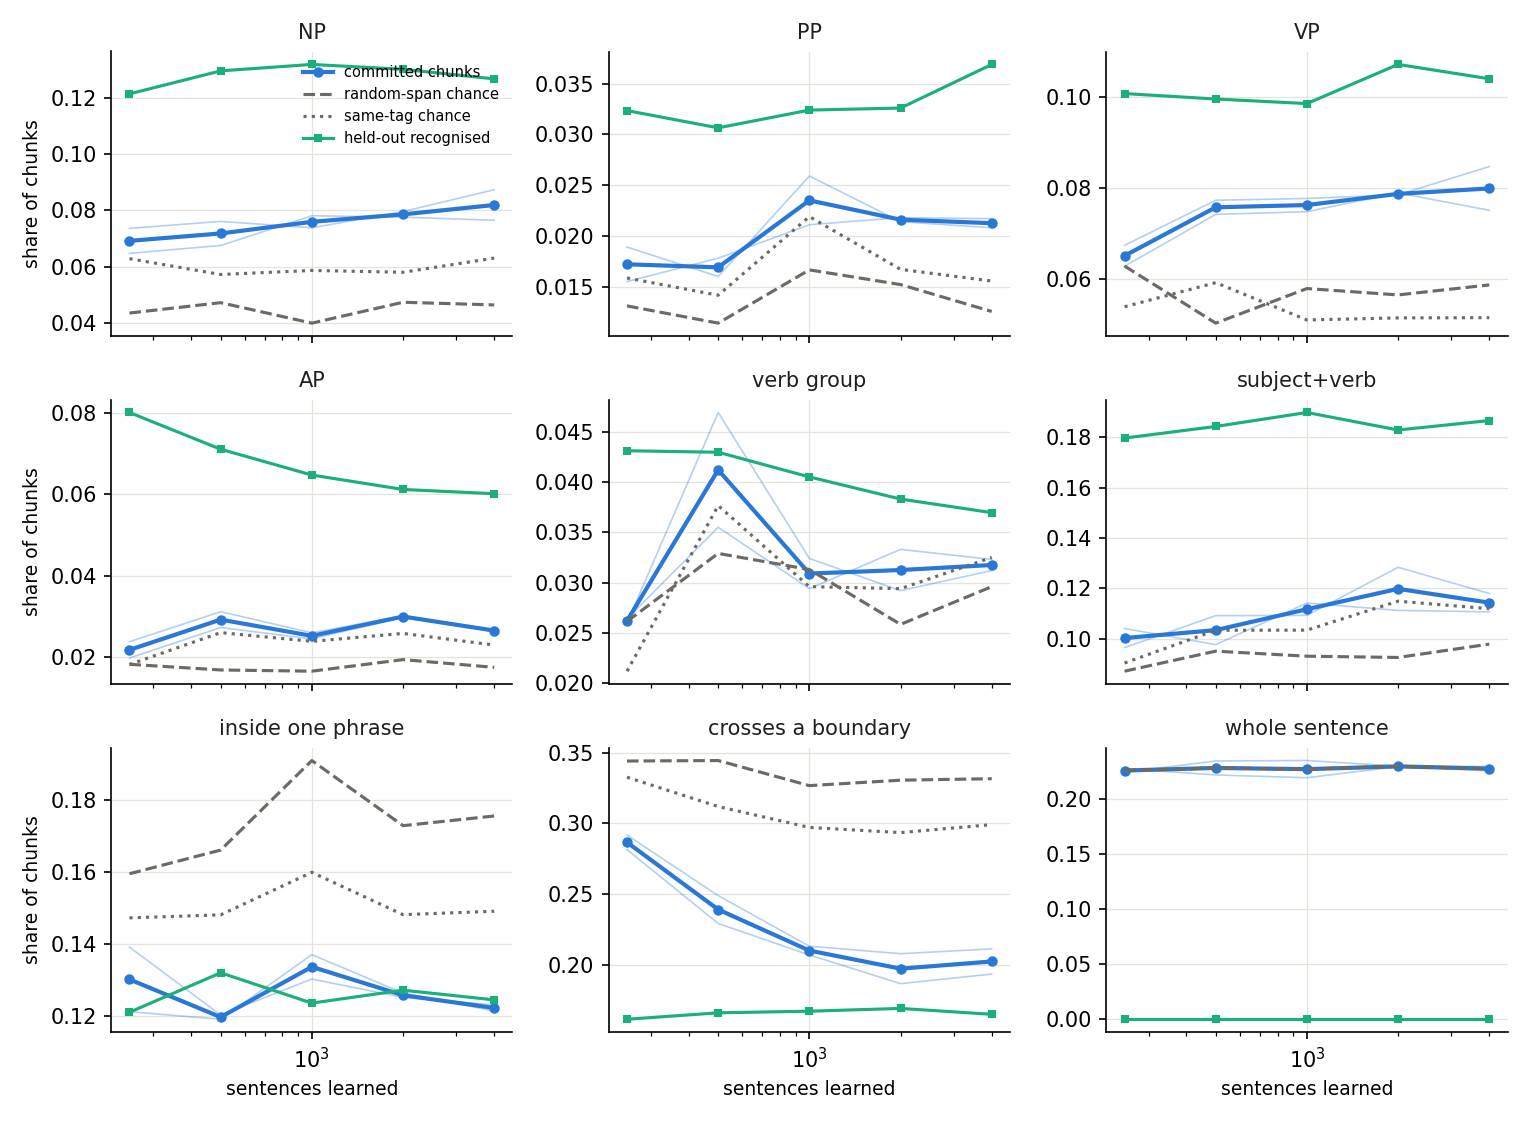
\includegraphics[width=0.8\textwidth]{figures/story_chunks_curves}
\caption{Share of committed chunks of each type against training sentences on TinyStories (blue; thin lines are seeds), where a committed chunk is a composite of the tree chosen during learning that the system stored as a record.
Dashed lines show random-span chance and dotted lines show chance for spans that start on a word of the same tag. The green line shows the share of recognized spans in held-out sentences.
Types come from the NLTK reference, and ``crosses a boundary'' marks chunks that straddle a reference phrase. The share of boundary-crossing chunks falls with experience.}
\label{fig:chunkcurves}
\end{figure}

\subsection{Generated sentences}

Table~\ref{tab:samples} lists the first two draws for three prompts after each model learned the same 1,000 sentences (seed 29, TinyStories).
Protocol: we show draws in the order sampled without selection, with the Qwen2.5-3B judge's probability that the sentence is grammatical, each model at its tuned temperature (\trellis{} with exact boundaries, temperature 2.0).
The prompt is the text each model receives before sampling, and the outputs show little visible dependence on it, so we read the draws as samples of each model's own behavior.
Each model writes new and fluent sentences next to word salad such as ``sara says good tim'' and ``they are very are friends.''
Over the whole run the share judged grammatical on seed 29 is .59 for \trellis{}, .58 for the LSTM, and .61 for the GPT.

\begin{table}[t]
\caption{The first two draws per prompt from each model after learning the same 1,000 TinyStories sentences (seed 29), with the Qwen2.5-3B judge's probability that the sentence is grammatical.
Draws appear in the order sampled, without selection. \trellis{} used the exact-boundary generator at temperature 2.0, and the LSTM and GPT used temperature .8.}
\label{tab:samples}
\begin{center}
\small
\begin{tabular}{p{0.14\textwidth}p{0.24\textwidth}p{0.24\textwidth}p{0.24\textwidth}}
\toprule
Prompt & \trellis{} & LSTM & GPT \\
\midrule
tom said sorry cat & it had a dog named spot (1.00) & the bird saw a big dog named max (1.00) & sara says good tim (0.00) \\
 & can play with it (0.04) & she is the best of you (0.01) & they were very happy (1.00) \\
he told his friends & tom and max were all day long (0.32) & mom said yes we can help (0.68) & tim and learned but sam was scared (0.03) \\
 & sue thought it and a big fish (0.05) & tim was happy and said thank you tim (0.00) & they are very are friends (0.00) \\
tim was very happy & it liked to help people (0.85) & max was not happy (1.00) & they were very happy (1.00) \\
 & let's go get your food together (0.99) & the bird felt sad (1.00) & tom and tim are friends (1.00) \\
\bottomrule
\end{tabular}
\end{center}
\end{table}

\subsection{Fair count of new grammatical sentences}

Figure~\ref{fig:gen} and Table~\ref{tab:gen} give the fair count for \trellis{} (configuration C1), the LSTM, and the GPT.
The eight-seed means show \trellis{} level with the LSTM at every size from 250 to 1,000 sentences and ahead of the GPT at 250 and 500 sentences, with 8 of 8 seeds won against the GPT at each of those sizes.
Against the LSTM \trellis{} wins on 5, 4, and 3 of 8 seeds at 250, 500, and 1,000 sentences.
At 4,000 sentences both neural models pull ahead, by .039 and .043 on the two seeds we ran, and the four confirmation seeds temper the headline.
On those four seeds alone, the advantage over the GPT is +.042 at 250 sentences (bootstrap interval [+.018, +.069], 4 of 4 seeds) and +.030 at 500 sentences ([+.013, +.052], 4 of 4).
The $t$ intervals on four seeds include zero at both sizes.
At 1,000 sentences the GPT leads \trellis{} on the confirmation seeds by .014 (bootstrap interval [$-$.027, $-$.001]; \trellis{} wins on 1 of 4 seeds). The claim that \trellis{} beats a matched GPT holds at 250 and 500 sentences, with weaker support on the confirmation seeds alone, and fails at 1,000.
%% PENDING r224: the judge for this comparison is being replaced or supplemented by a second judging (r224_rejudge.md); Table~\ref{tab:gen}, Figure~\ref{fig:gen}, and the paragraph above stay as written until that result arrives.

\begin{figure}[!t]
\centering
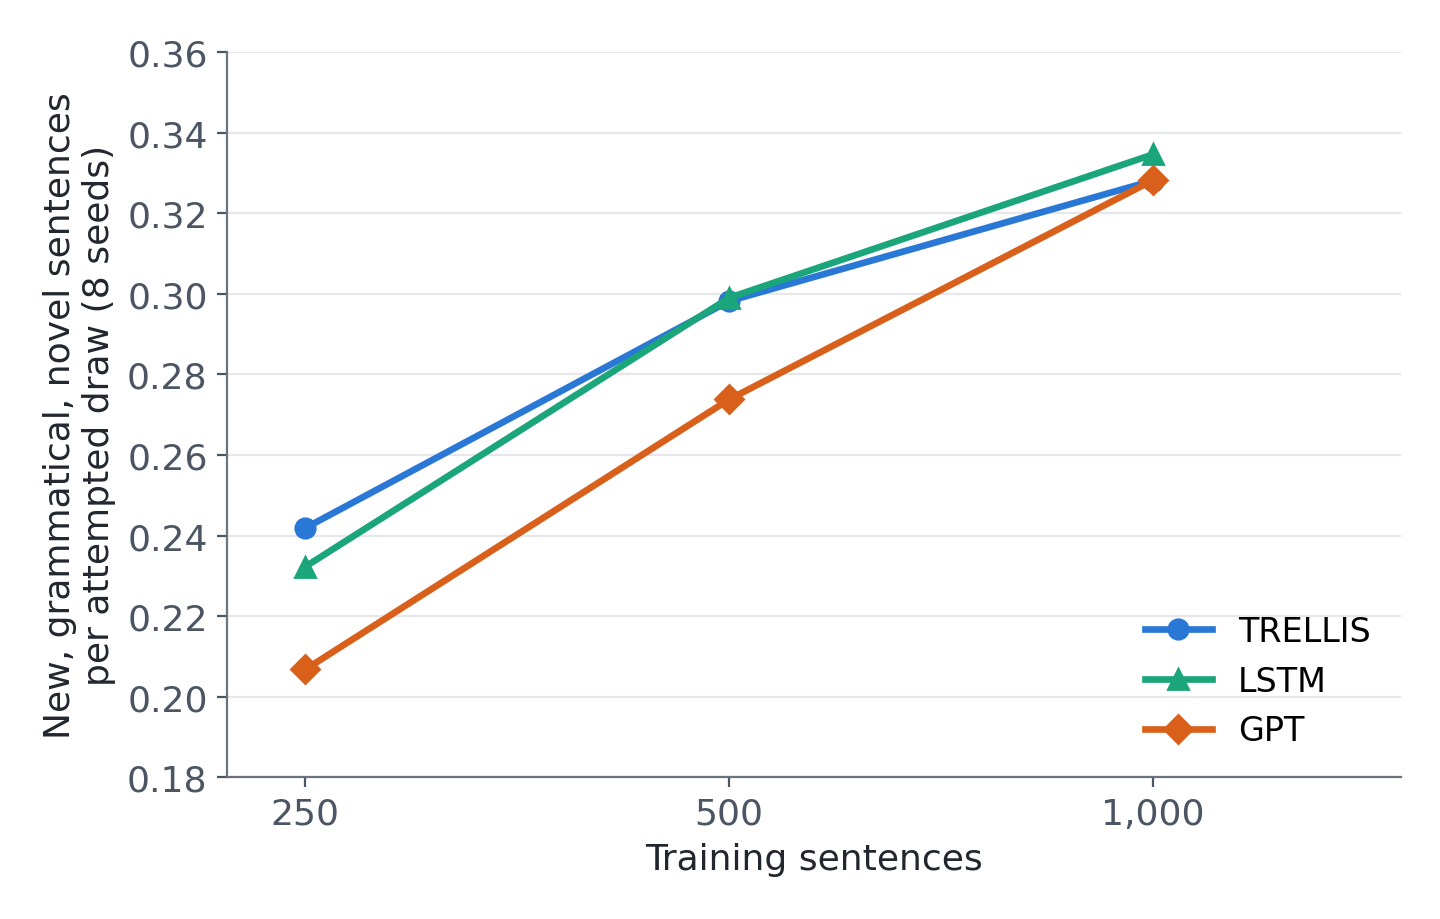
\includegraphics[width=0.62\textwidth]{figures/generation_fair_count}
\caption{Fair count (distinct, new, judged-grammatical sentences with an unstored trigram per attempted draw)
against training sentences for \trellis{}, an LSTM, and a GPT on TinyStories, each at its best sampling temperature.
Means over eight seeds at 250, 500, and 1,000 sentences. Judge: Qwen2.5-3B. The 4,000-sentence results appear in Table~\ref{tab:gen}.}
\label{fig:gen}
\end{figure}

\begin{table}[t]
\caption{Fair count on TinyStories sentences with the Qwen2.5-3B judge (configuration C1). Top block: mean over eight seeds with paired differences (mean, 95\% $t$ interval, seeds won).
Bottom block: the four confirmation seeds 29, 31, 37, and 41, which did not choose any setting, with paired differences (mean, 95\% bootstrap interval, seeds won).
The 4,000-sentence row uses seeds 13 and 17 only.}
\label{tab:gen}
\begin{center}
\footnotesize
\begin{tabular}{rcccll}
\toprule
$n$ & \trellis{} & LSTM & GPT & \trellis{} $-$ LSTM & \trellis{} $-$ GPT \\
\midrule
\multicolumn{6}{l}{\textit{All eight seeds}} \\
250   & .242 & .232 & .207 & +.010 [$-$.011, +.030], 5/8 & +.035 [+.016, +.054], 8/8 \\
500   & .298 & .299 & .274 & $-$.001 [$-$.013, +.011], 4/8 & +.024 [+.010, +.039], 8/8 \\
1,000 & .328 & .335 & .328 & $-$.007 [$-$.028, +.015], 3/8 & $-$.000 [$-$.023, +.022], 4/8 \\
4,000 & .319 & .358 & .362 & $-$.039, 0/2 & $-$.043, 0/2 \\
\midrule
\multicolumn{6}{l}{\textit{Four confirmation seeds}} \\
250   & .243 & .221 & .201 & +.022 [$-$.001, +.040], 3/4 & +.042 [+.018, +.069], 4/4 \\
500   & .295 & .294 & .265 & +.002 [$-$.006, +.011], 2/4 & +.030 [+.013, +.052], 4/4 \\
1,000 & .318 & .325 & .332 & $-$.007 [$-$.029, +.019], 1/4 & $-$.014 [$-$.027, $-$.001], 1/4 \\
\bottomrule
\end{tabular}
\end{center}
\end{table}

The tie comes from one design decision. The plain generator let a sentence start or end on a word that never starts or ends a stored sentence, and the judge accepted
many of these fragments. Reading the boundary exactly cuts the share of distinct outputs with an atypical boundary from .32--.42 to .07--.12 and lifts the fair count at 1,000 sentences from .316 to .338 on the four selection seeds.
A stricter count drops sentences whose first or last word never begins or ends a held-out sentence. Under it \trellis{} ties the LSTM and beats the GPT only at 250 sentences,
and it trails both models by about .014 at 1,000 sentences (Table~\ref{tab:strict}). On the eight-seed fair count, the lower bound of the $t$ interval against the LSTM is $-$.028 at 1,000 sentences, close to our $-$.03 margin.

\subsection{Novelty costs grammaticality}

A model that copies its training data writes grammatical sentences that are all stored, whereas a model that recombines parts freely writes new sentences and makes more errors. To compare models at matched novelty
we measure the share of new distinct sentences that contain a trigram unseen in training. Table~\ref{tab:novel} and Figure~\ref{fig:frontier} show that every learner pays for novelty with grammaticality.
At about a third novel, \trellis{} with a three-word window is grammatical .76 of the time and the LSTM .92. At about half novel the LSTM and GPT reach .81 and .80,
whereas \trellis{} with windows of four and five words reaches .71 and .67. Shorter windows copy more, and longer windows generalize more and err more.
These frontier runs use the plain \trellis{} generator (configuration C2, without the exact-boundary rule), and the headline generator in Table~\ref{tab:gen} sits elsewhere on the trade-off.

\begin{figure}[!t]
\centering
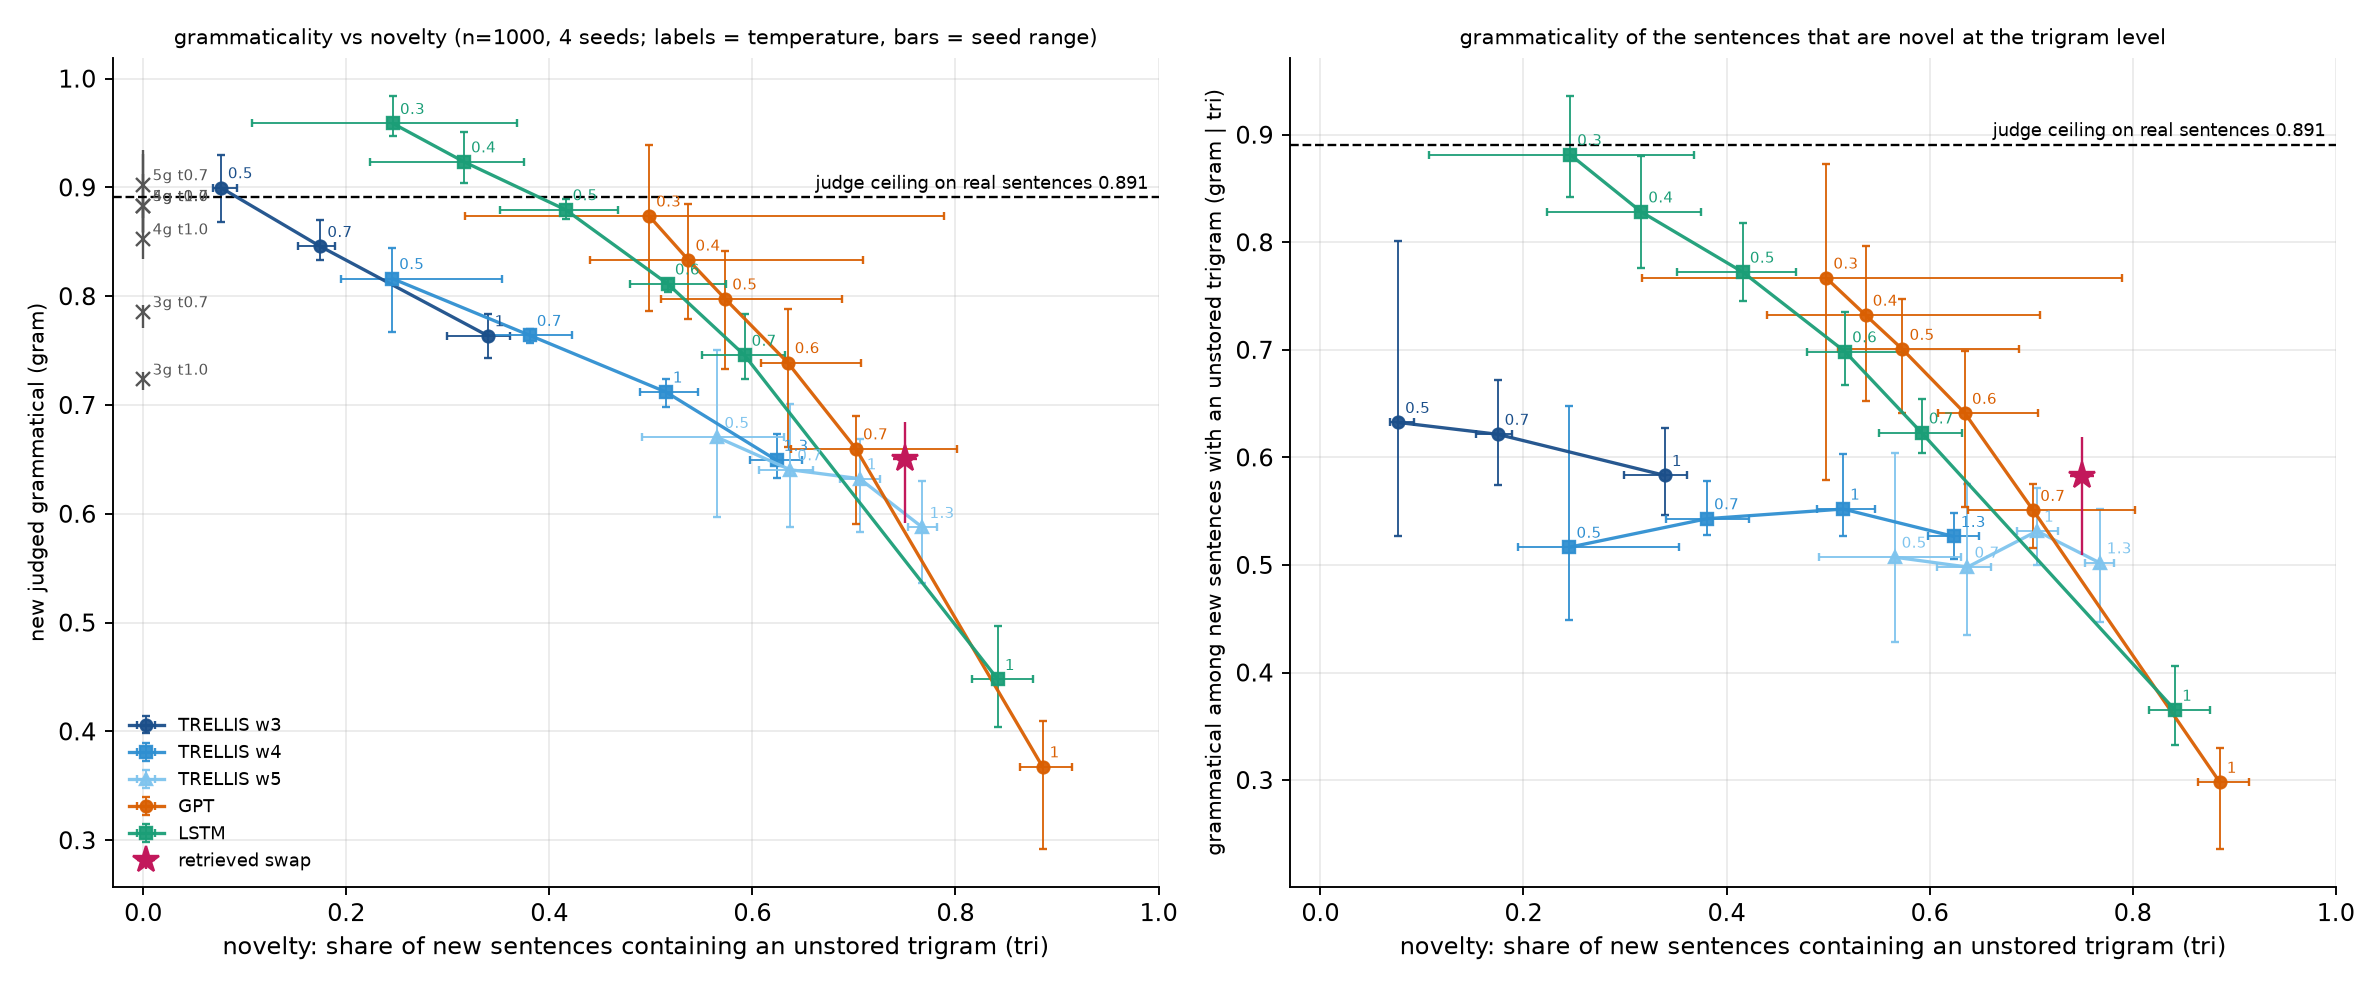
\includegraphics[width=\textwidth]{figures/story_frontier}
\caption{Grammaticality against novelty after 1,000 TinyStories sentences (four seeds; labels give sampling temperature, bars give the seed range; Qwen2.5-3B judge; configuration C2).
Novelty is the share of new distinct sentences containing a trigram unseen in training. Left, share of new sentences judged grammatical; right, grammaticality among the sentences that are novel at the trigram level.
The dashed line marks the judge's pass rate on real sentences (.891). Models: \trellis{} with windows of 3, 4, and 5 words, GPT, LSTM, and a reference generator that swaps one word in a retrieved training sentence (star).}
\label{fig:frontier}
\end{figure}

\subsection{Where \trellis{} falls behind}

From 1,000 to 4,000 sentences all three families write more distinct sentences, yet only \trellis{}'s new-trigram sentences become less grammatical (.464 to .410, against .50 for the LSTM and a rise from .487 to .570 for the GPT).
Real text and both neural models innovate after a history seen $k$ times at a rate that depends on $k$ alone. \trellis{} innovates too little after rare histories and too much after frequent ones, and
the imbalance grows with the amount of data. This diagnosis is a hypothesis, because the one attempt to correct the imbalance raised novelty without raising the fair count.
We estimate that a correction would recover .015 to .03 of fair count, which still leaves \trellis{} short of parity at 4,000 sentences.
Where a constraint of .90 grammaticality can be met, the LSTM keeps more novelty than \trellis{} (share of unstored trigrams .48 against .19). The tie holds at the fair-count optimum, where every model is .58 to .66 grammatical, but fails at the high-grammaticality end.
Judged with Qwen3-8B and phi-4 under a stricter prompt, no generator reaches .95 grammaticality among its distinct new sentences at 1,000 sentences.

\subsection{Real and broken sentences}

Two scores come from the memory. The parse score is the inside-pass log probability of the sentence per word. The generator score is the per-word log probability that the pair-gated generator assigns to each word given its left context.
Figure~\ref{fig:parsecurve} and Table~\ref{tab:parse} show the share of broken sentences each score accepts as training grows (configuration C4, set C).
The parse score alone accepts most scrambles at every size (.88 at 125 sentences, .77 at 4,000), and it accepts content-swapped sentences at .91 to .94, as a syntax checker should, because those sentences are grammatical.
The generator score does better. At 125 sentences it matches the GPT on scrambles (.39 against .40) and beats the LSTM (.65),
and by 500 sentences it trails the GPT (.19 against .09) while staying level with the LSTM (.16). It falls behind both by 4,000 sentences (.049 against .010 and .007). It is weakest on content swaps, where it still accepts .58 of them at 4,000 sentences against .41 and .40 for the neural models.
Every model in Table~\ref{tab:parse} rejects scrambles better than content swaps, so this pattern does not distinguish \trellis{}.
\trellis{} is worse than the neural models on both classes, and its parse carries little of the meaning information.

\begin{table}[t]
\caption{Share of broken held-out TinyStories sentences accepted by each score (configuration C4, set C: 300 real sentences per seed and their broken versions; four seeds), at the threshold that accepts 90\% of 400 real calibration sentences (lower is better).
\trellis{} parse is the inside-pass log probability per word, \trellis{} generator is the per-word log probability of the pair-gated generator, and LSTM and GPT are trained on the same sentences.
Real sentences are accepted .89 to .94 by every score.}
\label{tab:parse}
\begin{center}
\small
\begin{tabular}{llcccc}
\toprule
Broken class & Score & 125 & 500 & 1,000 & 4,000 \\
\midrule
Scrambled & \trellis{} parse & .88 & .81 & .78 & .77 \\
 & \trellis{} generator & .39 & .19 & .13 & .05 \\
 & LSTM / GPT & .65 / .40 & .16 / .09 & .08 / .04 & .01 / .01 \\
Adjacent swap & \trellis{} parse & .89 & .88 & .87 & .87 \\
 & \trellis{} generator & .75 & .69 & .64 & .53 \\
 & LSTM / GPT & .86 / .78 & .76 / .66 & .69 / .55 & .36 / .20 \\
Content swapped & \trellis{} parse & .94 & .93 & .92 & .91 \\
 & \trellis{} generator & .86 & .79 & .71 & .58 \\
 & LSTM / GPT & .80 / .80 & .66 / .70 & .62 / .64 & .41 / .40 \\
\bottomrule
\end{tabular}
\end{center}
\end{table}

\begin{figure}[!t]
\centering
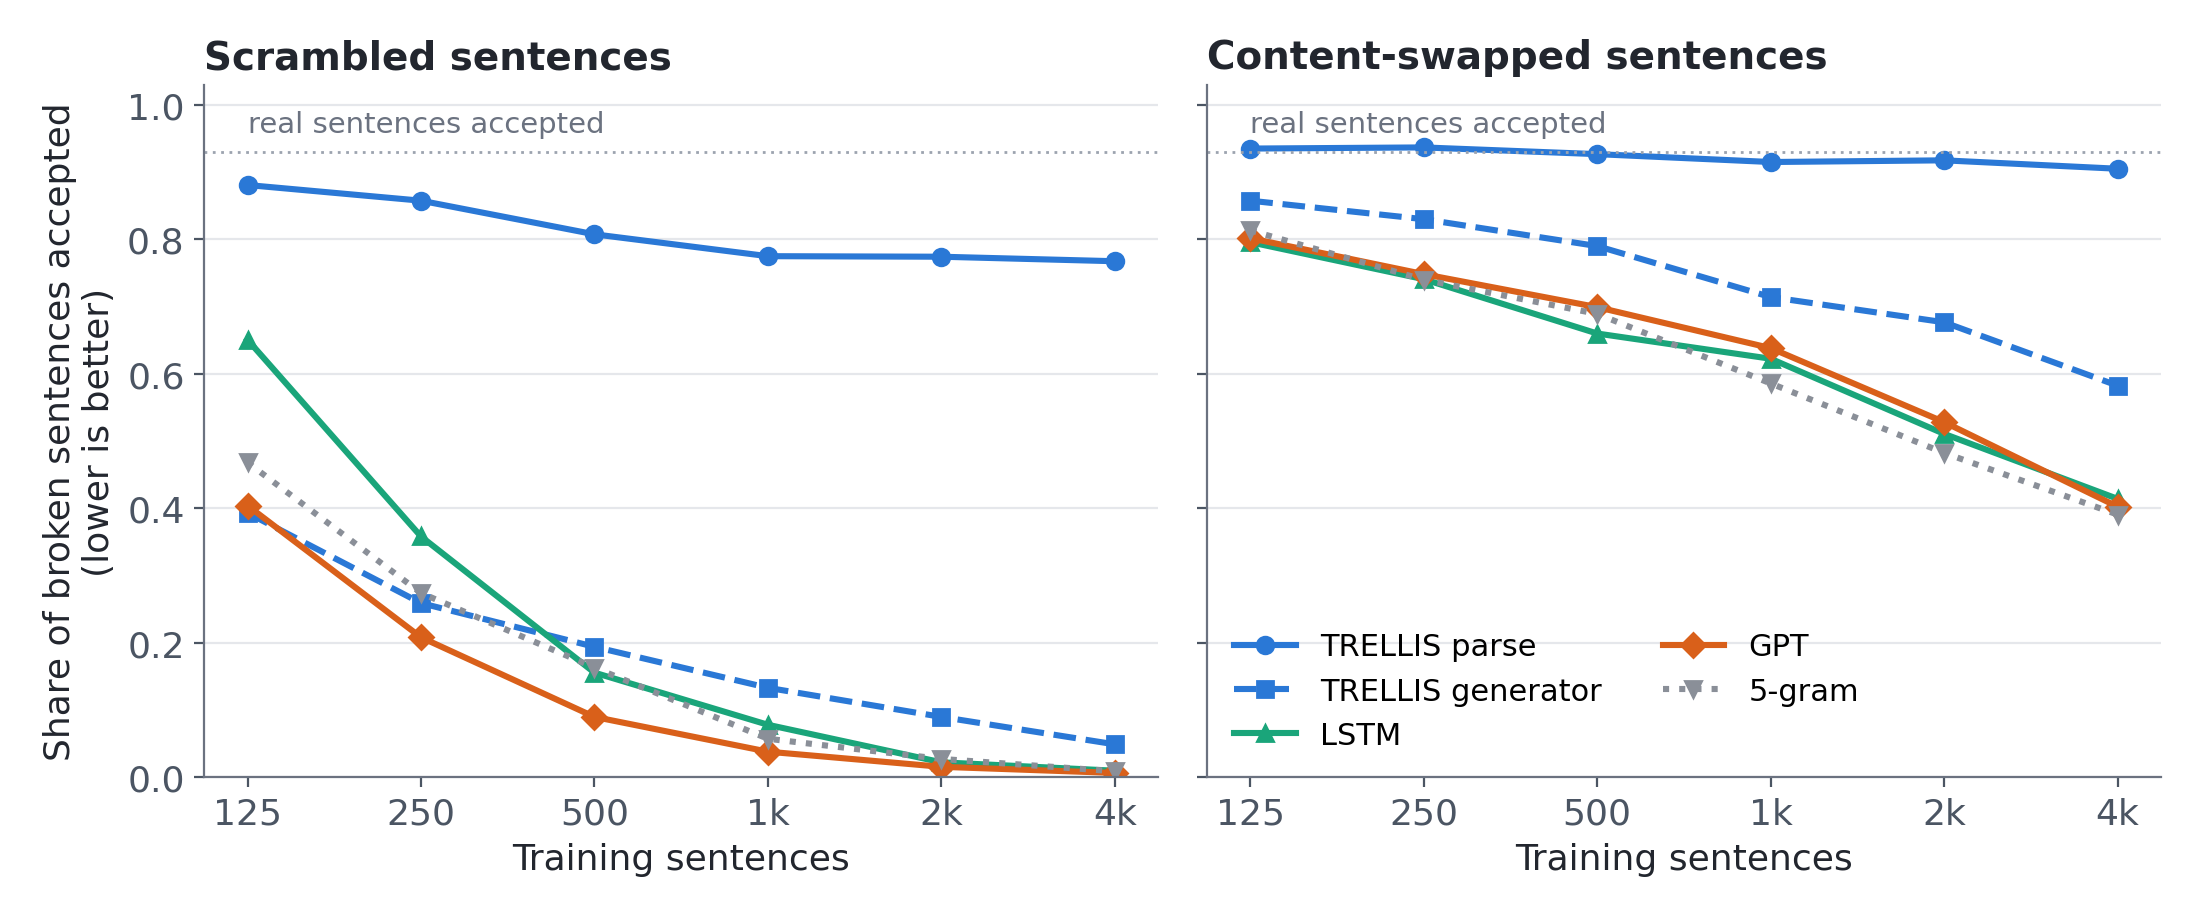
\includegraphics[width=\textwidth]{figures/parse_success_curve}
\caption{Share of broken held-out TinyStories sentences accepted by each score against training sentences (configuration C4, set C, four seeds). The threshold accepts 90\% of real calibration sentences,
so lower is better on every broken class. Parse and generator scores come from \trellis{}, and the LSTM and GPT train on the same sentences.}
\label{fig:parsecurve}
\end{figure}

A parser that is greedy and one that sums over every segmentation give the same answers on these sentences. Table~\ref{tab:window} shows that beam-one greedy parsing matches full inside-outside in F1 against the reference (.353 against .352) and in AUC for ungrammatical sentences (.541 against .542).
Of its trees, 93\% are identical to the full ones, and it costs .21 as much.
The first open question of version 1 has a negative answer on short sentences, and no experiment here tests longer ones.
%% PENDING r223: context abstraction (context-length ablation); see the delimited stub in the regimes section.

\section{Evaluation in Chess}

The same machinery runs on chess. \trellis{} knows nothing about the rules. A position is a set of pieces with their relations, and a chunk is a group of at most four pieces at relative offsets (the cap is a setting, configuration C5).
Figure~\ref{fig:chesstypes} shows frequent chunks from middle-game positions after learning, Figure~\ref{fig:chesscase} shows one held-out position as the parser reads it after 4,000 positions, and Figure~\ref{fig:chesscases} follows four positions through five training sizes.
Seven chunks hold 26 of the 27 pieces of the position in Figure~\ref{fig:chesscase}. The chunks include a castled king with the pawns f2, g2, and h2 (stored 861 times, the most common four-piece chunk), a pawn chain, and two rooks that defend each other.
Protocol: the system learns real positions in order, and at each checkpoint we parse held-out positions with learning off and outline the chunks whose recognition score clears a fixed threshold.

\begin{figure}[!t]
\centering
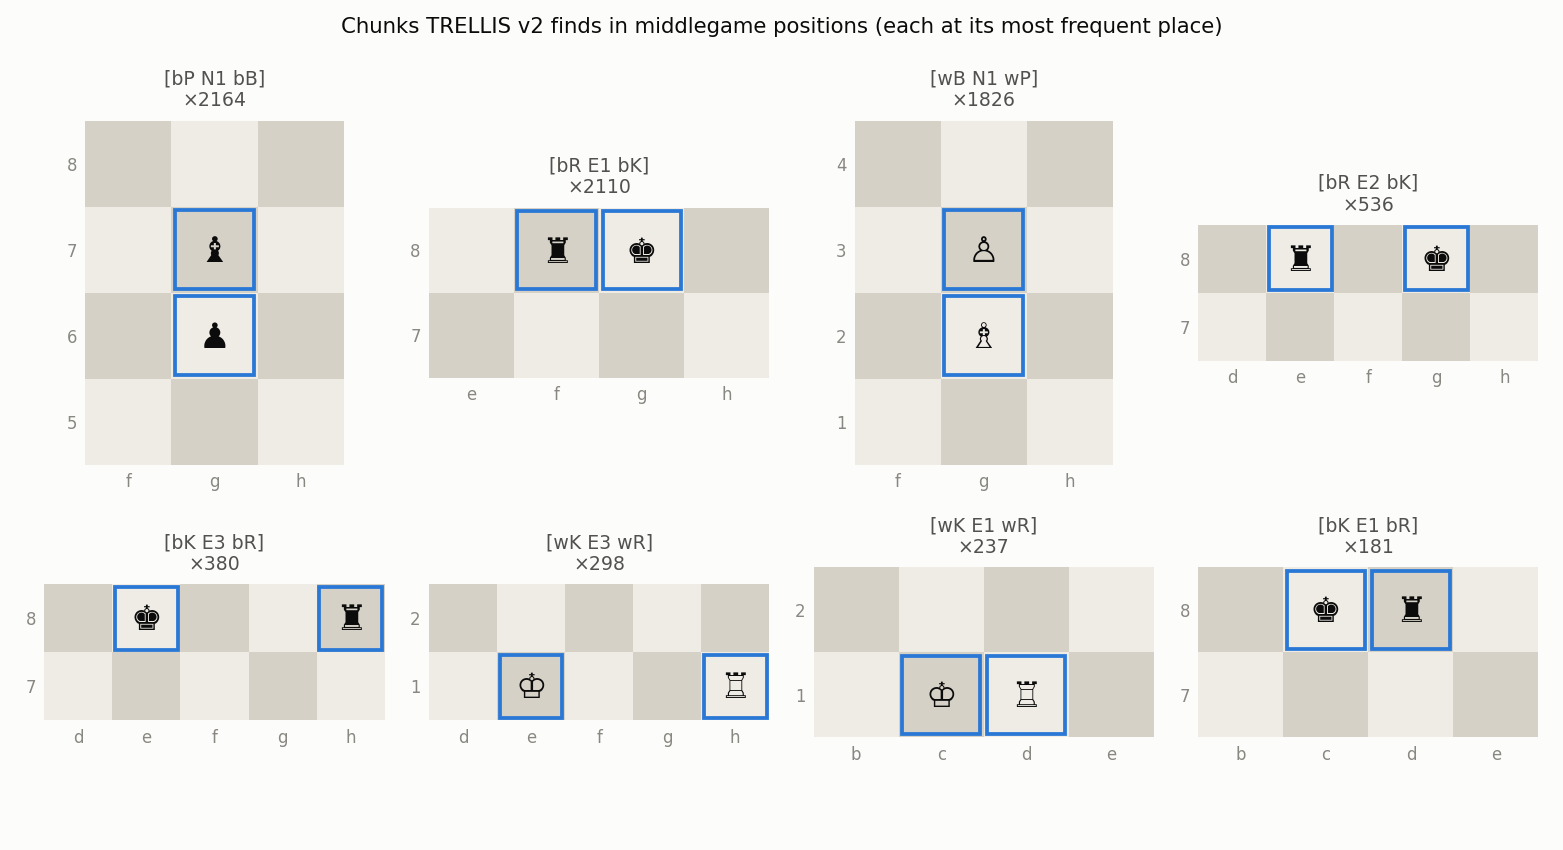
\includegraphics[width=0.85\textwidth]{figures/chess_chunk_types}
\caption{Frequent chunks that \trellis{} finds in Lichess middle-game positions, each drawn at its most frequent place, with its count. Labels give piece, offset, piece
(for example, \texttt{bR E1 bK} is a black rook and black king one file apart).}
\label{fig:chesstypes}
\end{figure}

\begin{figure}[!t]
\centering
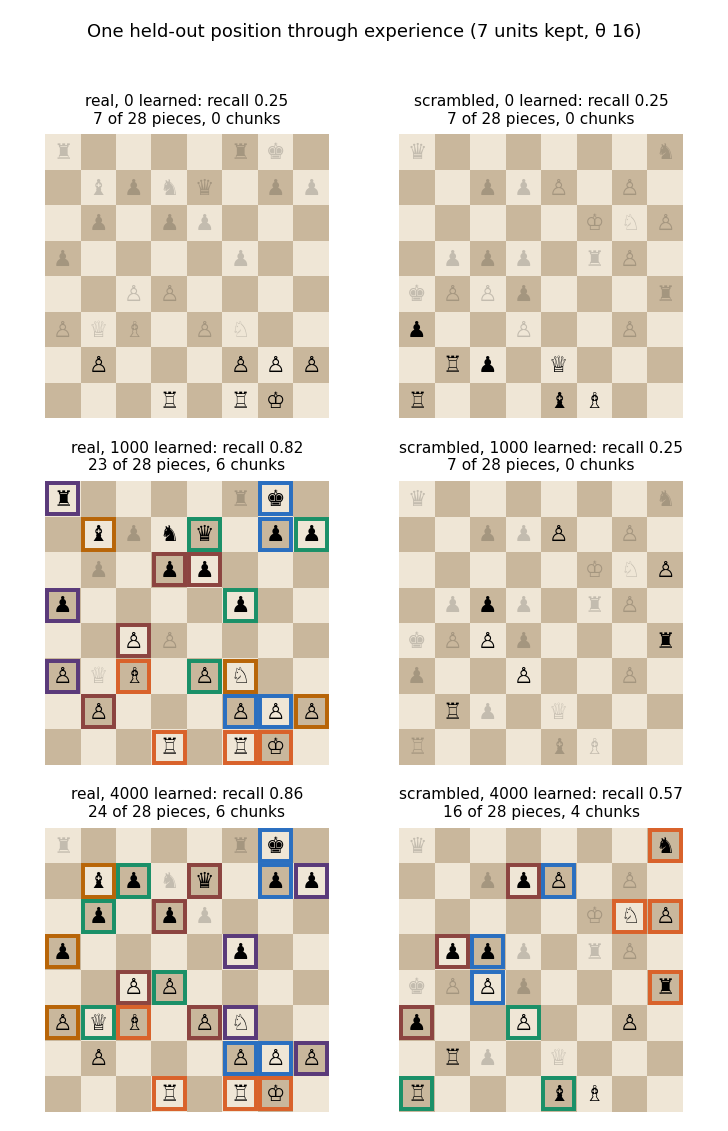
\includegraphics[width=0.45\textwidth]{figures/chess_case}
\caption{A held-out Lichess position as parsed by \trellis{} after 4,000 positions (seed 13). Seven chunks hold 26 of 27 pieces. The figure shows the parser's analysis of the position, and it comes from no recall trial.}
\label{fig:chesscase}
\end{figure}

\begin{figure}[!t]
\centering
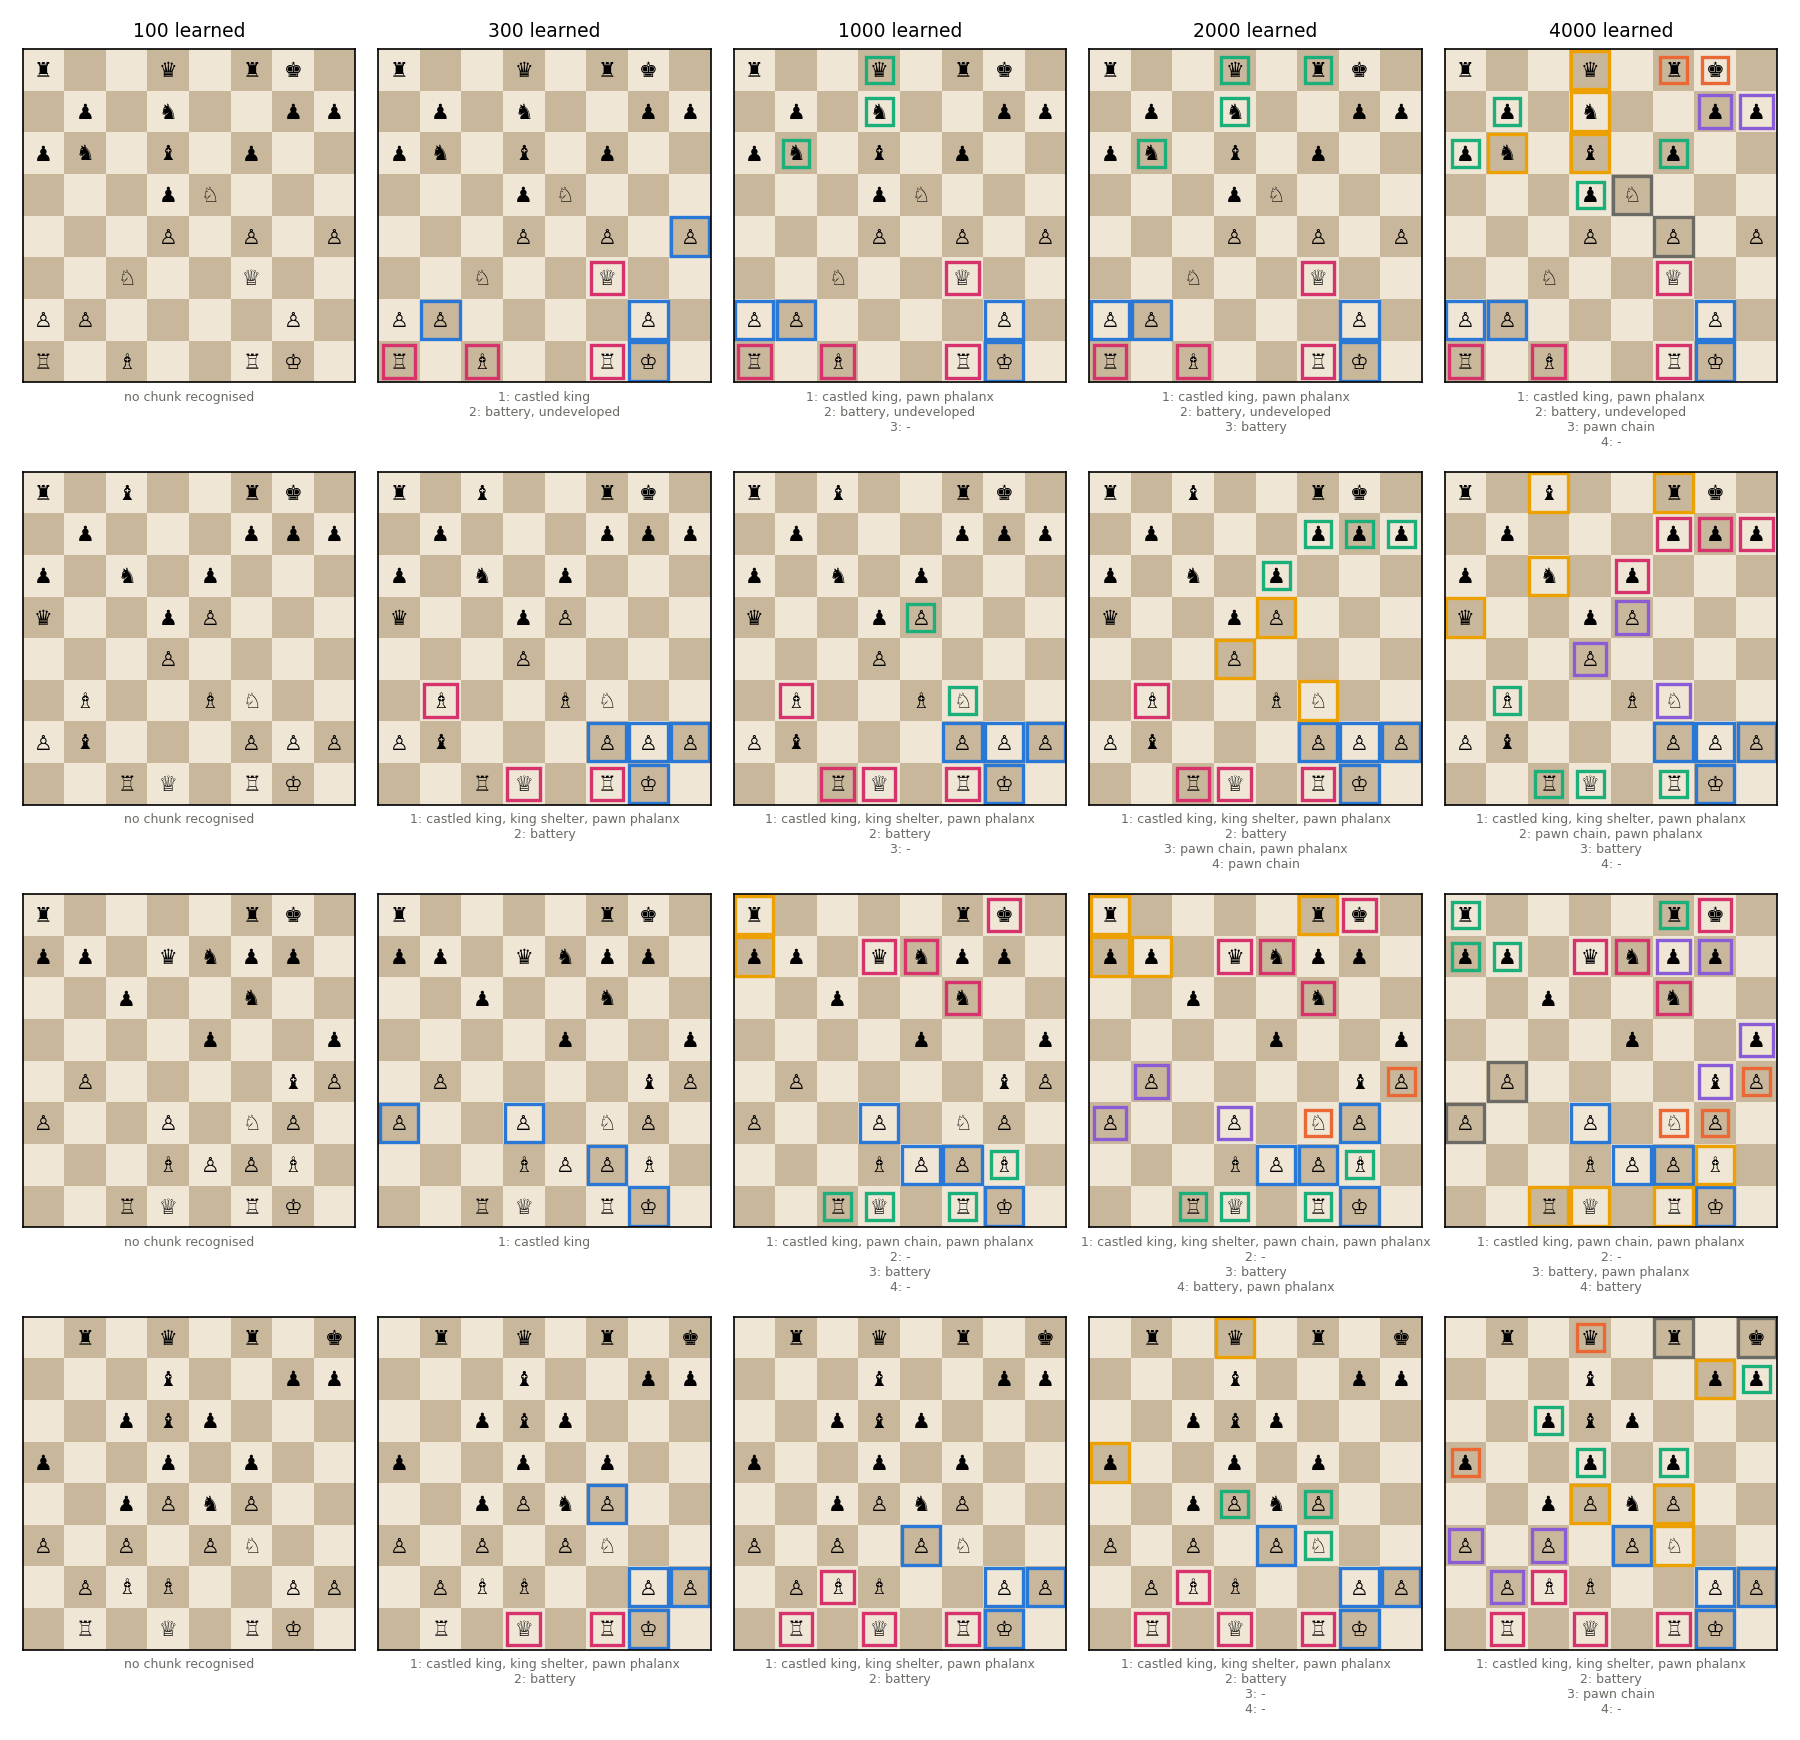
\includegraphics[width=0.95\textwidth]{figures/chess_ideas_cases}
\caption{Four held-out Lichess positions (rows) as \trellis{} parses them after learning 100, 300, 1,000, 2,000, and 4,000 positions (columns). Each outline marks one recognized chunk. Grey text lists the chess idea (rule-based label) carried by each of the first chunks,
and ``no chunk recognised'' means that no chunk cleared the recognition threshold. Lichess games, one learner.}
\label{fig:chesscases}
\end{figure}

\subsection{What the chess chunks encode}

We labeled each chunk with the chess ideas it contains and compared with groups of nearby pieces of the same size, over five seeds and 100 to 4,000 positions (Figure~\ref{fig:chessideas}).
Batteries appear at 2.5 to 2.7 times chance in the five-seed mean (2.2 to 3.2 across seeds), undeveloped back ranks at about 2 times, and pawn chains and phalanxes at up to about 1.8 times.
Pieces that attack each other (about 0.3 times) and rams (about 0.1 times) are split apart, which fits Chase and Simon's observation that attackers were rarely chunked with the pieces they attacked.
Castled kings (1.1 times) and fianchettos (0.9 to 1.1 times) sit near chance, and pieces defended by a pawn, a defence relation, appear at only 0.4 to 0.6 times chance.
Chase and Simon found defence relations common within a master's chunks, so the last result runs against their finding. The cap of four pieces may split larger formations, and the learned chunk that looks like a fianchetto (f7, g6, g8, h7) contains no bishop.

\begin{figure}[!t]
\centering
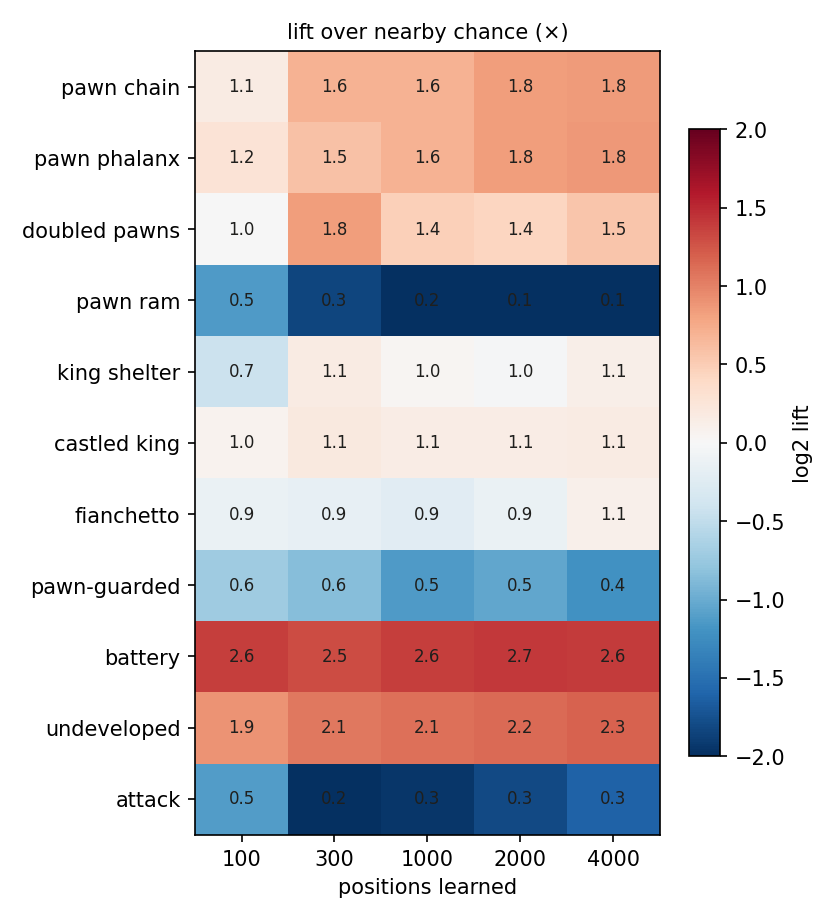
\includegraphics[width=0.45\textwidth]{figures/chess_ideas_lift}
\caption{Lift over nearby-piece chance of the share of recognized chunks that carry each chess idea, five-seed mean, positions from Lichess games.
Chance labels groups of nearby pieces of the same size as the chunks, so a lift above one means that memory prefers the idea.}
\label{fig:chessideas}
\end{figure}

\subsection{Compression of shifted positions}

If chunking is compression, the learned chunks should shorten the description of a held-out position. We code each of 1,000 held-out positions with the learned chunks, count bits, and compare with byte-pair coders over squares and over shapes, with Krimp, and with xz.
The model cost is not charged for any coder, so these numbers are held-out code lengths that leave out the model, unlike two-part description lengths. All numbers come from one seed (13) and one run per cell.
Table~\ref{tab:chess-bits} gives the result after 4,000 positions on four test sets.
Control positions resemble the training games, other openings and the other wing change the opening and the pawn structure, and shifted positions place shapes seen in training one file over, on squares that training never used.
On control positions byte-pair over squares is best, at 108.8 bits against 127.7 for the better of \trellis{}'s two arms and 130.6 for the recipe run.
On shifted positions, byte-pair over squares degrades to 205.5 bits. The recipe run of \trellis{} codes them in 153.6 bits, which saves 52 bits per position relative to byte-pair over squares, but it trails byte-pair over shapes (149.7) by about four bits.
A run with the \texttt{exact\_alone} setting off, which the recipe does not allow, reaches 147.2 and edges out byte-pair over shapes by 2.5 bits.
On other openings and the other wing, byte-pair over shapes beats the better \trellis{} arm by 16.9 and 13.4 bits. The advantage of relational chunks on shifted positions comes from describing chunks by shape, which a frequency-based miner can do too.
Figure~\ref{fig:chesscompress} shows the curves against positions learned.

\begin{table}[t]
\caption{Bits to code a held-out Lichess chess position after 4,000 training positions (lower is better; seed 13, 1,000 test positions per set, one run, model cost not charged).
Control positions come from games like the training games. Other openings and other wing change the opening and the pawn structure. Shifted positions place shapes seen in training one file over, on squares not seen in training.
\trellis{} (recipe) is the run with the system's recipe, available for control and shifted sets only. \trellis{} (best arm) is the better of the offsets-only and offsets-plus-squares arms in each column;
its shifted value, 147.2, comes from a run with \texttt{exact\_alone} off, which the recipe does not allow.}
\label{tab:chess-bits}
\begin{center}
\small
\begin{tabular}{lcccc}
\toprule
Coder & Control & Other openings & Other wing & Shifted \\
\midrule
\trellis{} (recipe) & 130.6 & -- & -- & 153.6 \\
\trellis{} (best arm) & 127.7 & 138.3 & 154.6 & 147.2 \\
Byte-pair over squares & 108.8 & 123.4 & 142.4 & 205.5 \\
Byte-pair over shapes & 111.3 & 121.4 & 141.2 & 149.7 \\
Krimp & 142.3 & 156.1 & 173.4 & 198.3 \\
xz & 122.7 & 132.2 & 153.0 & 181.3 \\
Piece-square list & 183.2 & 192.4 & 199.4 & 210.2 \\
\bottomrule
\end{tabular}
\end{center}
\end{table}

\begin{figure}[!t]
\centering
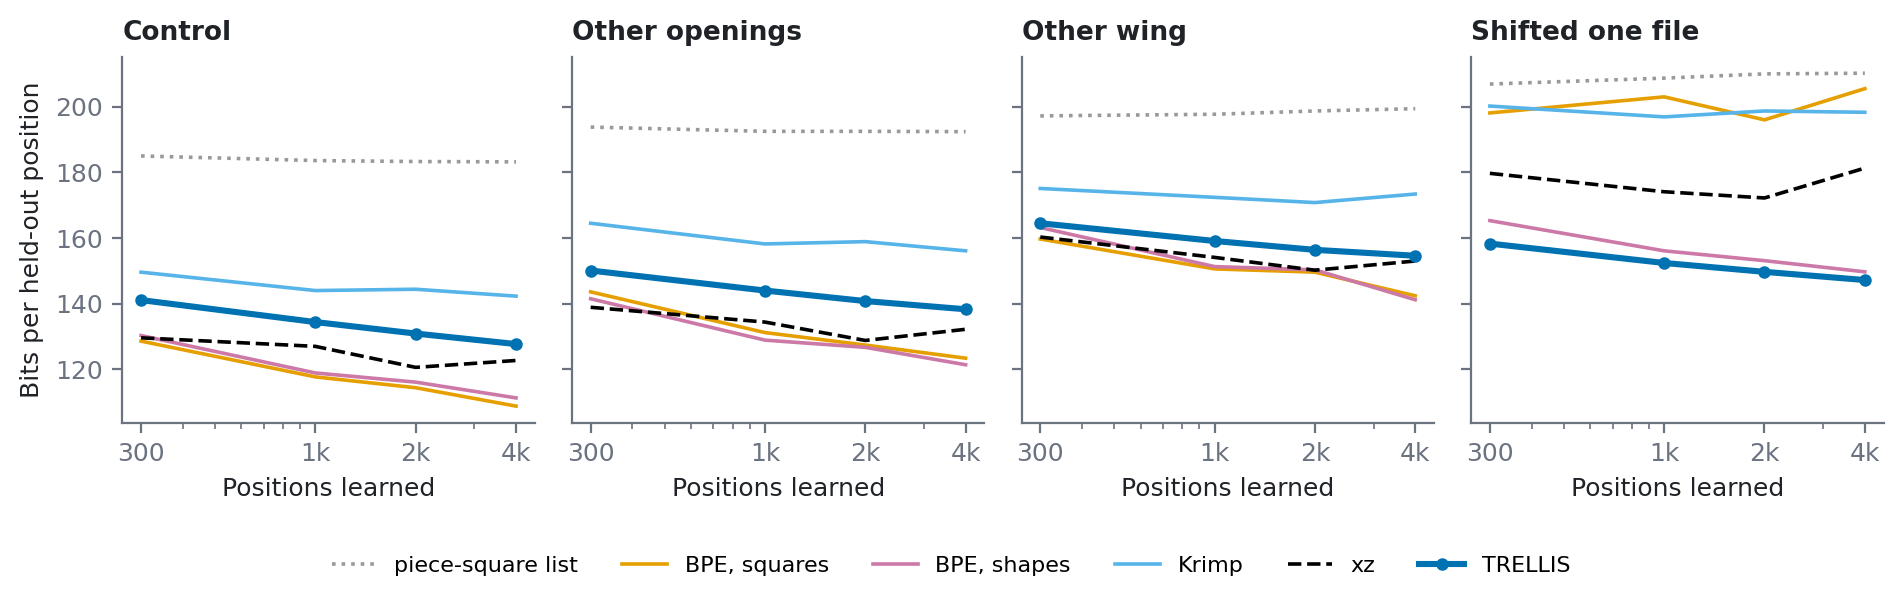
\includegraphics[width=\textwidth]{figures/chess_chunkers}
\caption{Bits per held-out Lichess position against positions learned (300 to 4,000) for \trellis{} and the comparison coders, on four test sets: control, other openings, other wing, and positions shifted one file (seed 13, model cost not charged).
\trellis{} here is the better of its two arms in each panel.}
\label{fig:chesscompress}
\end{figure}

\subsection{Chase and Simon recall}

Chase and Simon showed players a board for five seconds and asked them to rebuild it. Masters recalled far more pieces than beginners on real positions, and the difference shrank on random ones. We give \trellis{} a short-term memory of seven chunks
(or four, following the estimate of \citealp{cowan-magical-four}) and run the same task on Lichess middle-game positions with 24 to 26 pieces.
Protocol: the system parses the board, holds its recognized chunks in a store with the given number of slots, and rebuilds the position from them; further trials repeat the view with the previous reconstruction kept.
Table~\ref{tab:cstrial} shows one trial on one 26-piece position after 4,000 positions of learning (seed 13, seven slots, the first example saved for that run).
The first look yields 12 correct pieces from seven chunks, and later trials reach 18, 25, and 26 correct. The square d4 appears in two chunks, as a white pawn and as a white bishop, so one of the two is a commission error.

\begin{table}[t]
\caption{One Chase and Simon recall trial by \trellis{} on a 26-piece Lichess middle-game position (seed 13, 4,000 positions learned, seven chunk slots). Pieces are written square:piece with color prefix (w white, b black; K king, Q queen, R rook, B bishop, N knight, P pawn).
Pieces correct on trials 1 to 4: 12, 18, 25, 26.}
\label{tab:cstrial}
\begin{center}
\small
\begin{tabular}{cl}
\toprule
Slot & Chunk held after the first look \\
\midrule
1 & g1:wK, g2:wP, h2:wP, c2:wP \\
2 & a2:wP, c3:wN, b2:wP, d4:wP \\
3 & e1:wR \\
4 & h3:wR \\
5 & b4:bB \\
6 & d4:wB \\
7 & f4:wQ \\
\bottomrule
\end{tabular}
\end{center}
\end{table}

Table~\ref{tab:cs} gives first-trial recall across experience, averaged over three seeds with ten simulated subjects each. With seven slots, middle-game recall rises from 7.2 pieces after 300 positions to 9.7 after 1,000 and 12.9 after 4,000.
People recall 4, 8, and 16 pieces as beginners, club players, and masters, so the ordering matches but the values at the master point do not: with four slots the figure at 4,000 positions is 9.5.
On a longer stream with seven slots, recall reaches 15.6 on middle games at about 8,000 positions (two seeds, 16.2 and 14.9).
That approaches the master's 16 at twice the experience we fixed for the master in advance. Recall levels off near 16.7 at 16,000 positions and reaches about 17 at 27,459 positions on one seed (Figure~\ref{fig:cscurve}).
Recall is capped by the number of chunks times the pieces per chunk, so a better code raises it. With only four chunks recall reaches 11.0 and 11.1 at 8,000 and 16,000 positions, because a glance holds about 2.8 pieces.
Random positions diverge from the human pattern. With seven slots, first-trial recall on random positions rises from 4.2 to 5.5 to 6.0 over the three amounts of experience, and with four slots it rises from 2.2 to 2.8 to 3.2.
People fall from 3.0 to 2.5 to 2.0 across the same skill levels.
\citet{gobet-simon-random} found that skill still helps a little on random positions, which agrees in direction with our rise, though the 1973 values fall with skill.
Any learner that stores more chunks with more data would recall more, and we ran no chunker baseline, such as byte-pair chunks in the same slots, and no comparison with the recall simulations of CHREST \citep{gobet-simon-five-seconds}.
Ordering by experience alone is weak evidence for the account.

\begin{table}[t]
\caption{First-trial recall of pieces on Lichess middle-game, end-game, and random positions after \trellis{} learned 300, 1,000, and 4,000 positions (mean over three seeds, 13, 17, and 19, with ten simulated subjects each), with seven and four chunk slots,
next to people's recall \citep{chase-simon} as beginner, club player, and master. Random positions average the middle-game and end-game random sets (4.3 and 4.1 at 300 positions with seven slots).
The human values for random positions are as reported in the source and come from a single master, club player, and beginner.}
\label{tab:cs}
\begin{center}
\small
\begin{tabular}{llccc}
\toprule
Positions & Memory & 300 / beginner & 1,000 / club & 4,000 / master \\
\midrule
Middle game & \trellis{}, 7 slots & 7.2 & 9.7 & 12.9 \\
 & \trellis{}, 4 slots & 4.3 & 6.7 & 9.5 \\
 & People & 4 & 8 & 16 \\
End game & \trellis{}, 7 slots & 5.8 & 6.7 & 7.4 \\
 & \trellis{}, 4 slots & 3.4 & 3.9 & 4.5 \\
 & People & 4 & 7 & 8 \\
Random & \trellis{}, 7 slots & 4.2 & 5.5 & 6.0 \\
 & \trellis{}, 4 slots & 2.2 & 2.8 & 3.2 \\
 & People & 3.0 & 2.5 & 2.0 \\
\bottomrule
\end{tabular}
\end{center}
\end{table}

\begin{figure}[!t]
\centering
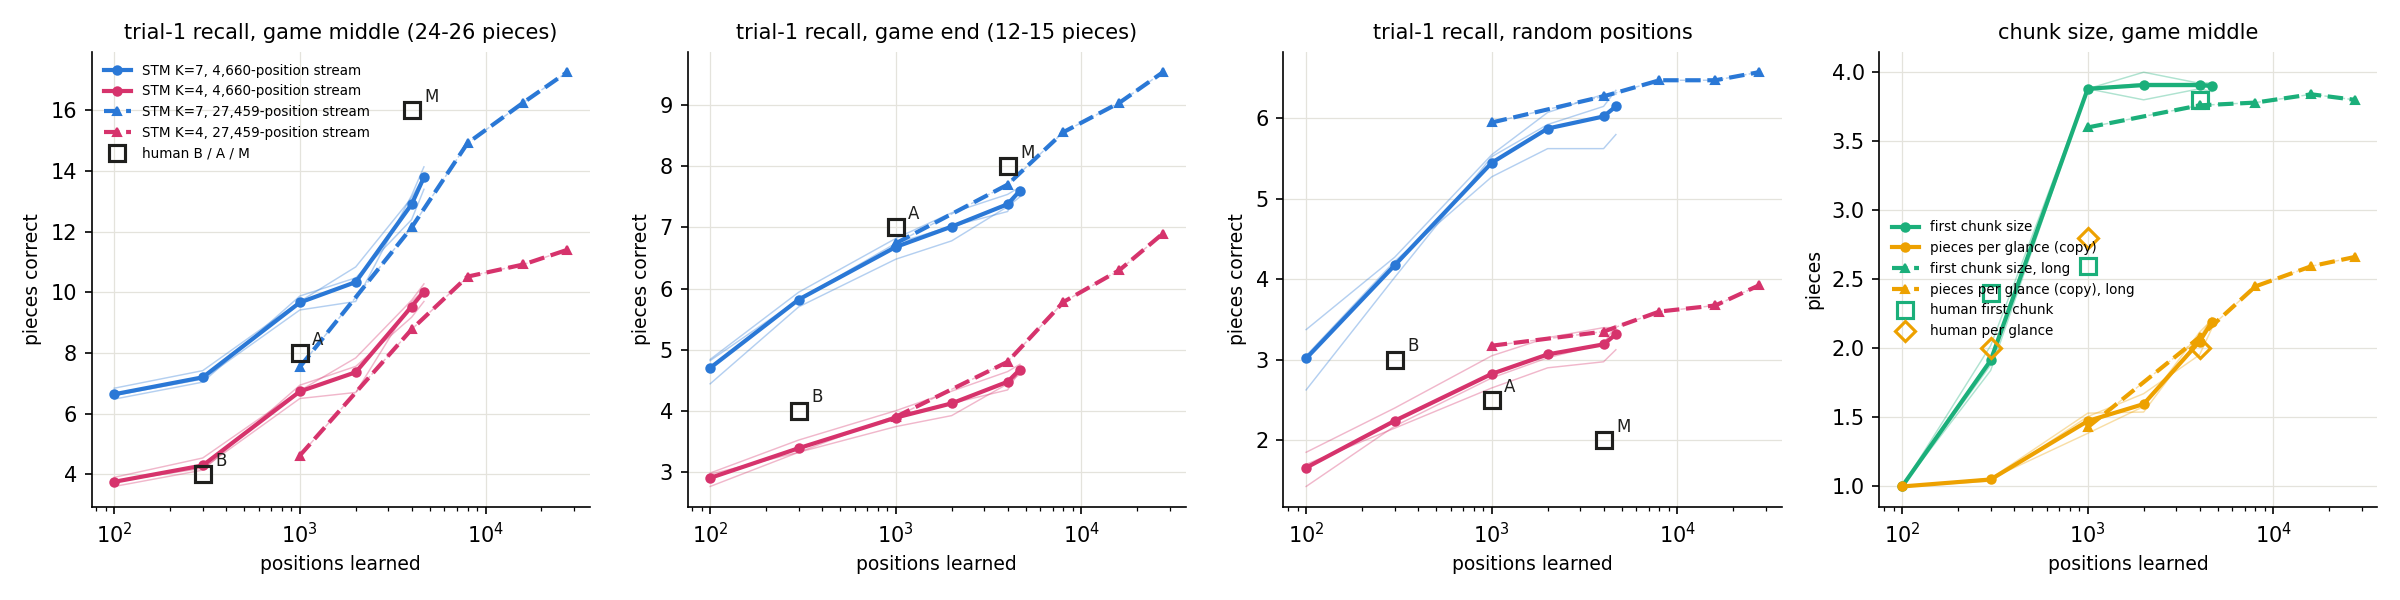
\includegraphics[width=\textwidth]{figures/chess_cs1973_curve}
\caption{Recall of Lichess middle-game, end-game, and random positions against positions learned (100 to 4,660 for solid lines, three seeds; 1,000 to 27,459 for dashed lines, the long stream), with seven and four chunk slots, next to the recall of people (black squares: beginner, class A, master).
The right panel shows the size of the first chunk and the pieces per glance in the copy task. Thin lines are single seeds.}
\label{fig:cscurve}
\end{figure}

\section{Meaningful, Syntax-Only, and Nonsense Output}

Language can be grammatical and meaningful, grammatical and meaningless, or neither. We asked whether one setting of \trellis{}, the abstraction of the words in the generator's context, moves the output among these three regimes.
We call them meaningful, syntax-only, and nonsense, and we define each by the questions the two-model judge passes. A sentence is meaningful if it passes both the syntax and the meaning question, syntax-only if it passes syntax and fails meaning, and nonsense if it fails syntax.
Producing the middle regime would show that the memory separates how words combine from their referents.

\paragraph{The judge can separate the regimes.} Table~\ref{tab:judge} shows that the ensemble passes syntax on .88 of held-out sentences whose content words we swapped within part of speech and passes meaning on only .13 of them, while it rejects scrambles and agreement errors on both questions.
On hand-built templates with the right frame, correct agreement, and absurd selection (for example, ``the boxes ate the flowers''), the syntax question passes every sentence, so the judge does not block the syntax-only regime.
Its known weakness is a single adjacent swap, which passes syntax at .13. The judge is validated on constructed controls only, and we did not hand-label generated sentences.

\paragraph{The dial reaches the two ends.} We read the generator's context at a chosen level $b$ of a word-category taxonomy that Cobweb builds from the neighbors of each word.
The leaf holds exact words, the root ($b=0$) holds one class, and larger $b$ gives finer classes.
Table~\ref{tab:regimecases} shows generated sentences at five levels after 4,000 sentences, labeled by the judge, and Table~\ref{tab:dial} gives the regime shares.
With exact words and the pair gate on, 63\% of the sentences are meaningful. With one class and no pair gate, 87\% to 89\% are nonsense. In between, the share of meaningful output falls
and the share of nonsense rises monotonically, and the syntax-only share stays between .08 and .27 with no interior peak.

\begin{table}[t]
\caption{Generated sentences labeled by the Qwen3-8B and phi-4 ensemble (meaningful, syntax-only, nonsense) at five abstraction levels of the generator (seed 13, 4,000 training sentences, window 5, temperature 1, pair gate on).
Draws are the first listed in the run, without selection. Level $b$ is the level of the word-category taxonomy that names the generator's context and its output classes, leaf meaning exact words.}
\label{tab:regimecases}
\begin{center}
\footnotesize
\begin{tabular}{llp{0.50\textwidth}}
\toprule
Level & Label & Sentence \\
\midrule
Leaf & meaningful & sue and tim were so happy; tom loved to play and run all day \\
 & syntax-only & she loved to give it back soon \\
 & nonsense & they learned to them \\
$b=7$ & meaningful & sue was pretty and scared; ben ran to tom \\
 & syntax-only & she went and said can i play too \\
 & nonsense & they had so every fun at the park \\
$b=6$ & meaningful & it was so big and proud; tom and bob wanted to play together \\
 & nonsense & it was a outside and said lily; do you want to play with back \\
$b=4$ & meaningful & lily and sam were friends \\
 & nonsense & he went to lot go idea; they felt again and boy to her \\
Root & nonsense & this had the this day be; they me friends \\
\bottomrule
\end{tabular}
\end{center}
\end{table}

\paragraph{The middle regime is not reached.} The largest syntax-only share over every setting, seed, and size is .265. We looked for the cause with oracles that need no model, and two oracle protocols appear in the results.
Protocol A (the first investigation) takes the meaningful sentences of the best generator and replaces every word outside the 50 most frequent word types with another type of the same class, with the judge deciding the result ($K=50$).
Under protocol A, classes from the learned word taxonomy leave at most .208 of the sentences syntax-only at 1,000 sentences, and .181 and .203 at 4,000 sentences on two seeds.
Part-of-speech classes give .199, .211, and .217, so the generators already sit at the level of this oracle.
Protocol B (the later investigation) protects no frequent types ($K=0$) and swaps only nouns, verbs, and adjectives. Under it, an oracle that swaps within exact morphosyntactic cells (tense, number, verb frame) reaches .45, .50, and .52 syntax-only on three runs,
and the same cells with the 50 most frequent types protected give .31 to .34 (Table~\ref{tab:oracle}). Protocol B supersedes the verdict of protocol A that substitution itself caps the regime: a clean syntax-only output exists when classes are fine and every content word is replaced.
Swapping across a coarse class breaks agreement and verb frames, which the judge treats as syntax failures, and about half of the part-of-speech swaps lose syntax for that reason.
More training text does not help, because the same 250-word vocabulary at 4,000 sentences leaves the ceiling at .18 to .22.

Class sources that need no labels fall short of the signature oracle under protocol B. The levels of the learned word taxonomy mix tags and frames, so only .4 to .5 of the members of a class share a morphosyntactic signature.
A later test added each word's own ending (its last one to three characters) and the nearest function words to the left and right as features of the word taxonomy, and it cut classes by size as well as by depth.
Every tree-class oracle stayed at a syntax-only share of .15 to .395 (typically .30 to .38), and class purity stayed at .4 to .58, so we did not build a generator that uses these classes.
A search for a read level of committed word occurrences (the level at which the context taxonomy is read) whose slots are pure in part of speech (at least .8) and varied (at least 3 bits of filler entropy) finds none. Purity reaches .8 only at the leaf, where filler entropy is .03 bits.
A feature that sees a verb's complement, or a tagging pass, would be a different mechanism, and we did not test one.

\subsection{Context length (pending)}
%% PENDING r223: context abstraction, which is the context-length ablation. Replace this stub with the result. Delimiter start.
This subsection will report how the width of the context window moves the regime shares at fixed abstraction. The result is pending and no number appears here.
%% PENDING r223: Delimiter end.

\paragraph{Chess shows no middle regime either.} We asked the same question of chess moves and of generated positions. \trellis{} plays the legal move after which memory recognizes the resulting position best. Among legal moves, the share that lose at least two pawns of material stays between .27 and .42 across
every setting. A uniformly random legal move loses that much .345 of the time on the same 200 positions, with a binomial interval of about $\pm.065$.
Recognition does not separate poor moves from reasonable ones (Table~\ref{tab:chessmoves}).
Generating whole positions from the chunk and concept distributions yields illegal boards at every level of the content taxonomy. Two seeds, 4,000 positions learned, and 500 boards per cell give a share of realistic legal boards of .085 at the leaf and .006 at the root, and the share of legal but unrealistic boards never exceeds .015.
A control that draws pieces independently from the training piece-square frequencies, with no chunks, scores .103, which equals or exceeds the leaf, so chunks do not help the realism of generated positions in this setting.
Recognition in \trellis{} does not encode legality, so a legal-but-poor regime does not appear.

\subsection{Parse then regenerate in chess (pending)}
%% PENDING r221: chess generation with piece counts and parse-then-regenerate. Replace this stub with the result. Delimiter start.
This subsection will report position generation with a piece-count facet and a regeneration test that parses a held-out position and resamples its chunks. The result is pending and no number appears here.
%% PENDING r221: Delimiter end.

\section{Related Research}

Several frameworks address parts of the problem. Labyrinth \citep{labyrinth-thompson-langley} encoded both primitive and composite concepts but lacked a context taxonomy and suffered substantial order effects, and Trestle \citep{trestle-maclellan} flattened its partonomic structure during processing.
\citet{maclellan-cobweb-language} adapted Cobweb to language modeling by describing each word through its neighbors, and our context taxonomy extends that representation.

EPAM \citep{feigenbaum-epam} and CHREST \citep{gobet-lane-chrest} build discrimination networks, and CHREST adds lateral links among chunks. \citet{gobet-simon-five-seconds} simulated expert recall with CHREST as a function of presentation time, and \citet{gobet-chunking-tics} reviewed chunking mechanisms in human learning.
These accounts treat chunks without a separate concept taxonomy and parse top down, and their recall simulations cover the same task as our Chase and Simon trial, which we ran without a CHREST baseline. Cowan \citeyearpar{cowan-magical-four} motivates our four-slot runs.

Grammar induction systems that minimize description length, such as that of \citet{wolff-grammar} and the simplicity-biased learner of \citet{grids-langley-stromsten}, learn a grammar, and so a code, by compression, and in that respect they share our principle.
Krimp \citep{vreeken-krimp} selects itemsets that minimize a two-part code, and we use it as a chess comparison. Byte-pair encoding \citep{sennrich-bpe} supplies the nearest compression baseline in both domains.
Models of child language such as the chunk-based learner of \citet{mccauley-cbl} and PARSER \citep{perruchet-parser} build chunks incrementally from the statistics of an input stream and test comprehension and production or segmentation.
Neither learns a concept taxonomy that names the parts of its chunks. The constituent-context model of \citet{klein-manning-ccm} induces bracketings from part-of-speech sequences, and the compound probabilistic context-free grammar of \citet{kim-compound-pcfg} induces them with neural parameterization and gradient training from words.
We have not compared \trellis{} with these systems. Our parser uses the inside-outside algorithm \citep{lari-young} and minimum-risk decoding \citep{goodman-metrics}. Neural language models are strong at scale and form no explicit chunks.

\section{Concluding Remarks}

We presented version 2 of \trellis{}, which learns chunks and concepts from raw streams without labels or gradients and parses and generates from one memory.
With little data it writes new grammatical sentences about as often as matched LSTM and GPT models, with the GPT result supported at 250 and 500 sentences only.
It falls behind both neural models as training data grow, its parse score alone is nearly blind to broken sentences, and it is weaker on meaning than on syntax. We do not claim that it competes with neural systems at their scale.
In chess its relational chunks match a shape-based byte-pair coder on shifted positions and lose to it on the other test sets.
Its recall of positions rises with experience in the order Chase and Simon found for people, and it rises on random positions as well, where people's recall does not.
No experiment here removes the content taxonomy, the context taxonomy, or the outside score from the generator, and the parse score adds nothing to the generator's discrimination, so we cannot attribute any language result to chunks.
The compression framing rests on the chess code lengths, which exclude model cost, and on the recall pattern.
%% PENDING r225: language compression result (held-out bits per token for TRELLIS, n-grams, BPE, neural models, with model description length) belongs in this paragraph.

Three questions remain open. Memory may choose the level of abstraction itself, so that no hand-set cut is needed and grammatical but meaningless output becomes reachable, but we have not shown it.
The full inside-outside computation may pay on longer inputs, which we did not test. A chess generator that composes positions from chunks while respecting the rules also remains to be built.

\begin{acknowledgements}
\noindent
The research reported here was supported by Grant No.\ FA9550-23-1-0580 from the US Air Force Office of Scientific Research, which is not responsible for its contents.
\end{acknowledgements}

{\parindent -10pt\leftskip 10pt\noindent
\bibliographystyle{cogsysapa}
\bibliography{refs}
}

\clearpage
\appendix

\section{Configurations of the System}

Table~\ref{tab:config} lists every configuration of \trellis{} that the paper uses. The configurations share the representation, taxonomies, and learning rule and differ in recipe options and in which read-out the result uses.

\begin{table}[h]
\caption{Configurations of \trellis{} used in each result. Seeds are TinyStories shuffles unless the row says chess. ``Edge-exact'' is the generator with the exact-boundary rule, and ``window'' is the generator's context window in words.}
\label{tab:config}
\begin{center}
\footnotesize
\begin{tabular}{p{0.05\textwidth}p{0.42\textwidth}p{0.40\textwidth}}
\toprule
Name & Setting & Results that use it \\
\midrule
C1 & Edge-exact generator, window 7 (250 and 1,000 sentences) or 6 (500), generation temperature 3.5, 2.8, 2.0 at 250, 500, 1,000 sentences; eight seeds; Qwen2.5-3B judge & Table~\ref{tab:gen}, Table~\ref{tab:strict}, Figure~\ref{fig:gen}, Table~\ref{tab:samples} \\
C2 & Plain generator without the exact-boundary rule, windows 3 to 5, temperatures .5 to 1; four seeds, 1,000 sentences & Table~\ref{tab:novel}, Figure~\ref{fig:frontier} \\
C3 & Learner of the generation recipe (posterior storage, content-only exact alone, window 7); parse read by default parser; four seeds, 250 to 1,000 sentences; set S & Table~\ref{tab:cases}, Table~\ref{tab:bio}, Table~\ref{tab:chunks}, Figures~\ref{fig:chunkcases} and \ref{fig:chunkcurves} \\
C4 & Learner recipe of the parsing-curve study (simpler candidate recipe); four seeds, 125 to 4,000 sentences; set C & Table~\ref{tab:parse}, Figure~\ref{fig:parsecurve}, Table~\ref{tab:window}, Table~\ref{tab:auc} \\
C5 & Chess recipe: relational chunks with at most four pieces, offsets plus squares and offsets only arms; seeds 13 (compression) and 13, 17, 19 (recall) & Table~\ref{tab:chess-bits}, Tables~\ref{tab:cstrial} and \ref{tab:cs}, Figures~\ref{fig:chesstypes} to \ref{fig:cscurve}, Table~\ref{tab:chessmoves} \\
C6 & Regime generator: gated token leaf with the pair gate, word taxonomy with function-word features, class gate and emission at level $b$, temperature .7 to 1, window 5 or 7; seeds 13 and 17 & Tables~\ref{tab:regimecases}, \ref{tab:dial}, and \ref{tab:oracle} \\
C7 & Chess compression run with \texttt{exact\_alone} off (not the recipe) & the shifted-set value 147.2 in Table~\ref{tab:chess-bits} \\
\bottomrule
\end{tabular}
\end{center}
\end{table}

\section{Generation Details}

Table~\ref{tab:strict} gives the boundary-strict count from the eight-seed run. The strict count drops distinct sentences whose first word never starts, or whose last word never ends, a real held-out sentence, for every family alike.
Under it \trellis{} matches the LSTM and beats the GPT only at 250 sentences, and at 1,000 sentences it trails both by about .014.
The rule for a match is a paired interval that includes zero with a lower bound above $-.03$. Under the $t$ interval, \trellis{} matches the LSTM at 500 sentences on the strict count, and under the bootstrap interval it does not.

\begin{table}[h]
\caption{Boundary-strict fair count on TinyStories, mean over eight seeds, with paired differences (mean, 95\% $t$ interval, seeds won). Judge: Qwen2.5-3B.}
\label{tab:strict}
\begin{center}
\footnotesize
\begin{tabular}{rcccll}
\toprule
$n$ & \trellis{} & LSTM & GPT & \trellis{} $-$ LSTM & \trellis{} $-$ GPT \\
\midrule
250   & .224 & .215 & .196 & +.008 [$-$.010, +.027], 5/8 & +.028 [+.010, +.045], 7/8 \\
500   & .273 & .282 & .262 & $-$.009 [$-$.021, +.002], 2/8 & +.011 [$-$.006, +.027], 5/8 \\
1,000 & .300 & .315 & .314 & $-$.014 [$-$.039, +.010], 2/8 & $-$.014 [$-$.036, +.009], 2/8 \\
\bottomrule
\end{tabular}
\end{center}
\end{table}

An earlier four-seed run found a GPT deficit of .014 at 1,000 sentences, and the four additional seeds did not replicate it, so the claim about the GPT holds at 250 and 500 sentences only.
The temperature grid for \trellis{} was extended after its optimum sat at the grid edge at 250 sentences, while the neural optima were interior. At 250 sentences the optimum later moved to temperatures of 4.0 to 4.5, and we report the pre-fixed value 3.5.
The pre-fixed setting for the eight-seed comparison came from the four selection seeds.
A judge ceiling applies: the judge passes about .89 of real held-out sentences, so no generator can exceed that grammaticality rate.

\begin{table}[h]
\caption{Share of new distinct sentences with a trigram unseen in training (new trigram) and share judged grammatical at matched novelty, after 1,000 TinyStories sentences (four seeds, Qwen2.5-3B judge, configuration C2, plain \trellis{} generator).
Real held-out sentences are judged grammatical .89 of the time. Each row is the setting whose novelty matches its partner.}
\label{tab:novel}
\begin{center}
\small
\begin{tabular}{lcc}
\toprule
Model & New trigram & Grammatical \\
\midrule
\trellis{}, window 3 & .34 & .76 \\
LSTM & .32 & .92 \\
\trellis{}, window 4 & .52 & .71 \\
LSTM & .52 & .81 \\
\trellis{}, window 5 & .57 & .67 \\
GPT & .57 & .80 \\
\bottomrule
\end{tabular}
\end{center}
\end{table}

\section{Windowed Parsing for Longer Inputs}

Full inside-outside cost grows cubically with sentence length, so we tested a spectrum between greedy parsing and full inside-outside at 1,000 sentences (four seeds, configuration C4, set C). A window variant runs inside-outside inside a window of $W$ symbols, freezes the best parse of its first $S$ symbols,
and moves on. A capped variant limits chunks to $2^D$ symbols per pass. Table~\ref{tab:window} gives selected cells. The sentences have at most eight tokens, so the cost saving here is modest (about a factor of two for the cap-four chart) and grows with length.
Disjoint windows hurt, because a chunk can never cross a window boundary in the pass that creates it, whereas overlapping windows that commit only the first part of the window recover full-parser accuracy against the shallow-phrase reference.
No variant changes acceptance of broken sentences by more than seed noise, so these scores cannot discriminate between parsers.
We keep full inside-outside for the sentences in this paper. The asymptotic gain of the cap-four chart is arithmetic, and we did not measure it on long sentences.

\begin{table}[h]
\caption{Windowed and capped inside-outside parsing on TinyStories after 1,000 sentences (configuration C4, set C, mean over four seeds). Cost is composites evaluated per sentence relative to full parsing; F1 is against the NLTK shallow-phrase reference
(right-branching scores .423 on the same sentences); ``same as full'' is F1 between the variant's trees and full-parse trees.}
\label{tab:window}
\begin{center}
\small
\begin{tabular}{lcccc}
\toprule
Variant & Cost & F1 vs.\ reference & Same as full & Mean AUC, ungrammatical \\
\midrule
Full inside-outside & 1.00 & .352 & 1.00 & .542 \\
Greedy (beam 1) & .21 & .353 & .934 & .541 \\
Cap-four chart & .53 & .362 & .970 & .542 \\
Window 4, stride 2 & .48 & .413 & .799 & .540 \\
Window 3, stride 2 & .30 & .428 & .788 & .538 \\
Window 4, disjoint & .31 & .308 & .854 & .541 \\
Window 3, disjoint & .21 & .242 & .557 & .558 \\
\bottomrule
\end{tabular}
\end{center}
\end{table}

\section{Further Metric Tables}

Table~\ref{tab:auc} reports the area under the curve (AUC) with which each score separates real held-out sentences from each broken class, at 125 and 4,000 sentences (configuration C4, set C, four seeds).
The generator score keeps pace with the baselines on scrambles at 125 sentences and trails them at 4,000, and its content-swap AUC at 4,000 sentences is .81 against .88 to .89 for the n-gram, LSTM, and GPT. The parse score is near chance on every class.

\begin{table}[h]
\caption{AUC for real versus broken held-out TinyStories sentences (configuration C4, set C, four seeds) for the per-word parse score and generator score of \trellis{} and for the 5-gram, LSTM, and GPT trained on the same sentences.}
\label{tab:auc}
\begin{center}
\small
\begin{tabular}{lcccc}
\toprule
Score & \multicolumn{2}{c}{125 sentences} & \multicolumn{2}{c}{4,000 sentences} \\
 & Scramble & Content swap & Scramble & Content swap \\
\midrule
\trellis{} parse & .537 & .475 & .641 & .517 \\
\trellis{} generator & .886 & .613 & .981 & .810 \\
5-gram & .880 & .702 & .993 & .887 \\
LSTM & .807 & .694 & .993 & .886 \\
GPT & .888 & .682 & .995 & .880 \\
\bottomrule
\end{tabular}
\end{center}
\end{table}

\begin{table}[h]
\caption{Chunk statistics after 1,000 TinyStories sentences (configuration C3, four seeds, set S; no confidence intervals, seed ranges only). Overlap is the Jaccard overlap of the 50 most frequent chunks between seeds;
F1 is bracket F1 against the NLTK shallow-phrase reference on each seed's held-out sentences.}
\label{tab:chunks}
\begin{center}
\small
\begin{tabular}{lc}
\toprule
Statistic & Value \\
\midrule
Top-50 chunk overlap across seeds, \trellis{} & .33 \\
Top-50 overlap, raw n-gram frequency / byte-pair encoding & .51 / .43 \\
Chunks in the top 50 of all four seeds & 14 \\
Held-out parses that differ from right-branching & .82 \\
Held-out parses that are neither right- nor left-branching & .66 \\
F1 against reference, \trellis{} (four seeds) & .32 -- .39 \\
F1 against reference, right-branching & .49 \\
\bottomrule
\end{tabular}
\end{center}
\end{table}

\begin{table}[h]
\caption{Share of control sentences passed by the Qwen3-8B and phi-4 ensemble on the syntax and meaning questions (test half, 150 sentences per class, built from held-out TinyStories sentences).
The content-word swap here is the ensemble study's own, built with animacy and emotion flips and listed verb frames, and differs from the tag-based swap of the broken-sentence studies.}
\label{tab:judge}
\begin{center}
\small
\begin{tabular}{llcc}
\toprule
Control class & Example & Syntax pass & Meaning pass \\
\midrule
Real & the fish was not happy anymore & 1.00 & .95 \\
Content words swapped & the hard door looked hard & .88 & .13 \\
Two adjacent words swapped & little the bird looked sad & .13 & .06 \\
Agreement error & they is not friends anymore & .04 & .15 \\
Scrambled & not anymore was happy the fish & .02 & .00 \\
\bottomrule
\end{tabular}
\end{center}
\end{table}

\begin{table}[h]
\caption{Share of generated TinyStories sentences in each regime (judge: Qwen3-8B and phi-4 ensemble; configuration C6) as the generator's context moves from exact words (leaf) to one class (root), seed 13 after 1,000 and 4,000 sentences and seed 17 after 4,000.
Meaningful passes syntax and meaning, syntax-only passes syntax alone, and nonsense fails syntax. The leaf row is the leaf setting with the highest meaningful share (window 7 at 1,000 sentences and window 5 at 4,000, temperature .7).
Class levels use a taxonomy built from function-word features and a class-level pair gate. Entries are meaningful / syntax-only / nonsense.}
\label{tab:dial}
\begin{center}
\footnotesize
\begin{tabular}{lccc}
\toprule
Setting & 1,000, seed 13 & 4,000, seed 13 & 4,000, seed 17 \\
\midrule
Leaf, pair gate on & .630 / .170 / .201 & .634 / .176 / .190 & .621 / .182 / .197 \\
Class level $b=7$ & .331 / .255 / .415 & .293 / .211 / .497 & .323 / .265 / .412 \\
Class level $b=6$ & .197 / .208 / .595 & .180 / .161 / .658 & .201 / .225 / .574 \\
Class level $b=4$ & .107 / .140 / .753 & .087 / .116 / .797 & .116 / .157 / .727 \\
Root (one class) & .034 / .095 / .871 & .029 / .082 / .889 & .033 / .083 / .885 \\
\bottomrule
\end{tabular}
\end{center}
\end{table}

\begin{table}[h]
\caption{Share of oracle sentences that are syntax-only under the two oracle protocols (judge: Qwen3-8B and phi-4 ensemble). Both start from the meaningful sentences of the gated-leaf generator and swap words within a class.
Protocol A protects the 50 most frequent word types ($K=50$) and swaps every other word. Protocol B protects none ($K=0$) and swaps nouns, verbs, and adjectives. Values are for 1,000 sentences on seed 13, and 4,000 sentences on seeds 13 and 17.}
\label{tab:oracle}
\begin{center}
\small
\begin{tabular}{llccc}
\toprule
Protocol & Classes & 1,000, s13 & 4,000, s13 & 4,000, s17 \\
\midrule
A ($K=50$) & learned word taxonomy & .208 & .181 & .203 \\
A ($K=50$) & part of speech & .199 & .211 & .217 \\
A ($K=50$) & morphosyntactic cells & .31 & .33 & .34 \\
B ($K=0$) & morphosyntactic cells & .45 & .50 & .52 \\
B ($K=0$) & learned word taxonomy, best cell & -- & .349 & .395 \\
\bottomrule
\end{tabular}
\end{center}
\end{table}

\begin{table}[h]
\caption{Chess move quality for 200 Lichess positions at ply 30 after \trellis{} learned 1,000 positions (seed 13). The legal-move rows choose among legal moves; the displacement rows add 120 random piece displacements per position.
Sound moves lose less than two pawns of material by a fixed capture search. Real game continuations are sound .983 of the time on 300 validation positions, random legal moves .697, and worst legal moves .033.
Binomial uncertainty on 200 positions is about $\pm.065$.}
\label{tab:chessmoves}
\begin{center}
\small
\begin{tabular}{lccc}
\toprule
Candidates and choice & Sound & Legal but losing & Illegal \\
\midrule
Legal moves, best recognized & .625 & .375 & 0 \\
Legal moves, uniform random & .655 & .345 & 0 \\
Any displacement, best recognized & .125 & .105 & .770 \\
\bottomrule
\end{tabular}
\end{center}
\end{table}

When the candidates include random piece displacements, so the model is not told the rules, about three quarters of the candidates are illegal, and the best-recognized pick is illegal .77 of the time against .70 for a random pick.
The material criterion catches hung pieces and lost exchanges and does not capture positional sense.

\end{document}
